\documentclass[10pt,a4paper]{article}

% --- Paquetes de configuración regional y tipografía ---
\usepackage[utf8]{inputenc}
\usepackage[T1]{fontenc}
\usepackage[spanish,es-tabla,es-noshorthands]{babel}
\usepackage{lmodern}
\usepackage{microtype}

% --- Geometría y márgenes optimizados para máximo 15 páginas ---
\usepackage[a4paper,top=1.6cm,bottom=1.6cm,left=1.5cm,right=1.5cm,headheight=13pt,footskip=18pt]{geometry}

% --- Elementos gráficos y tablas ---
\usepackage{graphicx}
\graphicspath{{images/}{./}}
\usepackage{xcolor}
\usepackage{booktabs}
\usepackage{tabularx}
\usepackage{colortbl}
\usepackage{float}
\usepackage{caption}
\usepackage{subcaption}
\usepackage{amsmath,amssymb}
\usepackage{tikz}
\usetikzlibrary{shapes.geometric, arrows.meta, positioning, fit, backgrounds, babel}

% --- Espaciados compactos ---
\setlength{\parskip}{1.8pt plus 0.6pt minus 0.4pt}
\setlength{\intextsep}{3pt plus 1pt minus 1pt}
\setlength{\textfloatsep}{4pt plus 1pt minus 1pt}
\setlength{\floatsep}{3pt plus 1pt minus 1pt}

% --- Estilo de encabezados y pies de página ---
\usepackage{fancyhdr}
\usepackage{lastpage}
\usepackage{titlesec}
\usepackage{enumitem}
\setlist{topsep=1.5pt, itemsep=1.0pt, parsep=0pt, partopsep=0pt}
\renewcommand{\arraystretch}{0.96}

% --- Cajas estilizadas y código ---
\usepackage{tcolorbox}
\tcbuselibrary{skins,breakable,listings}
\usepackage{listings}
\usepackage{multicol}

% --- Hipervínculos ---
\usepackage{hyperref}

% --- Definición de Paleta de Colores Institucional ---
\definecolor{uncblue}{RGB}{10, 48, 92}        % Azul Institucional FCEFyN
\definecolor{primary}{RGB}{18, 52, 86}         % Azul oscuro principal
\definecolor{accentteal}{RGB}{0, 136, 145}     % Teal acento
\definecolor{darkslate}{RGB}{33, 37, 41}       % Texto principal
\definecolor{termbg}{RGB}{17, 24, 39}          % Fondo terminal oscuro (slate 900)
\definecolor{termfg}{RGB}{243, 244, 246}       % Texto terminal blanco nítido
\definecolor{boxbg}{RGB}{248, 250, 252}        % Fondo cajas
\definecolor{boxborder}{RGB}{203, 213, 225}    % Borde cajas
\definecolor{tableheader}{RGB}{226, 232, 240}  % Fondo encabezado tablas
\definecolor{rowalt}{RGB}{248, 250, 252}       % Filas alternas
\definecolor{notebg}{RGB}{239, 246, 255}       % Fondo notas
\definecolor{noteborder}{RGB}{59, 130, 246}    % Borde notas
\definecolor{codecomment}{RGB}{100, 116, 139}  % Comentarios código
\definecolor{codekeyword}{RGB}{14, 116, 144}   % Keywords C/Bash

% --- Configuración de Hipervínculos ---
\hypersetup{
    colorlinks=true,
    linkcolor=uncblue,
    citecolor=uncblue,
    urlcolor=accentteal,
    pdftitle={Informe Técnico — TP2: Registro Central NEXUS},
    pdfauthor={Grupo Infostealer - FCEFyN UNC},
    pdfsubject={Sistemas Operativos I - Trabajo Práctico Nro 2}
}

% --- Configuración de Encabezados y Pies de Página ---
\pagestyle{fancy}
\fancyhf{}
\fancyhead[L]{\footnotesize\scshape\color{primary}Sistemas Operativos I — TP N$^\circ$ 2: Registro Central NEXUS}
\fancyhead[R]{\footnotesize\scshape\color{uncblue}Capítulo 2 · Daemon nexusd}
\fancyfoot[L]{\scriptsize\color{darkslate!70}FCEFyN — Universidad Nacional de Córdoba}
\fancyfoot[R]{\footnotesize\bfseries\color{primary}Página \thepage\ de \pageref{LastPage}}
\renewcommand{\headrulewidth}{0.5pt}
\renewcommand{\footrulewidth}{0.3pt}

% --- Configuración de Títulos de Sección Compactos ---
\titleformat{\section}
  {\normalsize\bfseries\color{uncblue}}
  {\thesection.}{0.5em}{}[\titlerule]
\titlespacing*{\section}{0pt}{1.0ex plus 0.2ex minus .1ex}{0.35ex plus .1ex}

\titleformat{\subsection}
  {\small\bfseries\color{primary}}
  {\thesubsection.}{0.4em}{}
\titlespacing*{\subsection}{0pt}{0.7ex plus 0.2ex minus .1ex}{0.25ex plus .1ex}

\titleformat{\subsubsection}
  {\footnotesize\bfseries\color{accentteal}}
  {\thesubsubsection.}{0.3em}{}
\titlespacing*{\subsubsection}{0pt}{0.5ex plus 0.1ex minus .1ex}{0.2ex plus .1ex}

% --- Configuración de Entornos de Terminal y Cajas ---
\newtcblisting{terminalbox}[2][]{
    enhanced,
    colback=termbg,
    colframe=uncblue!90,
    coltitle=white,
    title={\scriptsize\bfseries\texttt{\detokenize{#2}}},
    arc=1.5mm,
    boxrule=0.7pt,
    left=2.0mm,
    right=2.0mm,
    top=1.0mm,
    bottom=1.0mm,
    before skip=2.0pt,
    after skip=2.0pt,
    listing only,
    listing options={
        backgroundcolor=\color{termbg},
        frame=none,
        rulecolor=\color{termbg},
        basicstyle=\scriptsize\ttfamily\bfseries\color{white},
        breaklines=true,
        columns=flexible,
        keepspaces=true,
        extendedchars=true,
        inputencoding=utf8,
        literate={á}{{\'a}}1 {é}{{\'e}}1 {í}{{\'i}}1 {ó}{{\'o}}1 {ú}{{\'u}}1 {ñ}{{\~n}}1 {Á}{{\'A}}1 {É}{{\'E}}1 {Í}{{\'I}}1 {Ó}{{\'O}}1 {Ú}{{\'U}}1 {Ñ}{{\~N}}1 {¿}{{?`}}1 {¡}{{!`}}1 {—}{{\textemdash}}1 {─}{{-}}1
    },
    #1
}

\newtcolorbox{pregunta}[1]{
    enhanced,
    breakable,
    colback=boxbg,
    colframe=uncblue!75,
    fonttitle=\footnotesize\bfseries\color{white},
    title={Pregunta de Investigación: #1},
    arc=1.2mm,
    boxrule=0.5pt,
    left=2.0mm,
    right=2.0mm,
    top=0.7mm,
    bottom=0.7mm,
    before skip=1.5pt,
    after skip=1.5pt
}

\newtcolorbox{notabox}[1][Nota Técnica]{
    enhanced,
    breakable,
    colback=notebg,
    colframe=uncblue,
    coltitle=white,
    fonttitle=\footnotesize\bfseries\color{white},
    title={\textbf{#1}},
    arc=1.2mm,
    boxrule=0.6pt,
    left=2.0mm,
    right=2.0mm,
    top=1.0mm,
    bottom=1.0mm,
    before skip=2.0pt,
    after skip=2.0pt
}

\lstset{
    basicstyle=\scriptsize\ttfamily\color{darkslate},
    keywordstyle=\bfseries\color{uncblue},
    stringstyle=\color{accentteal},
    commentstyle=\itshape\color{codecomment},
    backgroundcolor=\color{boxbg},
    frame=single,
    rulecolor=\color{boxborder},
    breaklines=true,
    breakatwhitespace=true,
    tabsize=4,
    showstringspaces=false,
    inputencoding=utf8,
    extendedchars=true,
    literate={á}{{\'a}}1 {é}{{\'e}}1 {í}{{\'i}}1 {ó}{{\'o}}1 {ú}{{\'u}}1 {ñ}{{\~n}}1 {Á}{{\'A}}1 {É}{{\'E}}1 {Í}{{\'I}}1 {Ó}{{\'O}}1 {Ú}{{\'U}}1 {Ñ}{{\~N}}1 {¿}{{?`}}1 {¡}{{!`}}1 {—}{{\textemdash}}1 {─}{{-}}1
}

\begin{document}

% ==============================================================================
% PORTADA INSTITUCIONAL
% ==============================================================================
\begin{titlepage}
    \hypersetup{pageanchor=false}
    \centering
    \vspace*{-1cm}
    
    \begin{figure}[H]
        \centering
        
\includegraphics[width=0.28\textwidth]{logo_unc.png}
    \end{figure}
    
    \vspace{0.1cm}
    {\large\scshape\bfseries UNIVERSIDAD NACIONAL DE CÓRDOBA}\\[0.1cm]
    {\large\scshape FACULTAD DE CIENCIAS EXACTAS, FÍSICAS Y NATURALES}\\[0.15cm]
    {\normalsize\scshape DEPARTAMENTO DE COMPUTACIÓN}\\[0.35cm]
    
    \rule{\linewidth}{1.2pt}\\[0.25cm]
    {\LARGE\bfseries\color{uncblue} SISTEMAS OPERATIVOS I}\\[0.15cm]
    {\Large\bfseries\color{primary} Trabajo Práctico Nro 2: “Registro Central NEXUS”}\\[0.12cm]
    {\large\itshape\color{accentteal} Capítulo 2 · Daemon de Sistema, Persistencia e Integración de Servicios}
    \rule{\linewidth}{1.2pt}\\[0.5cm]
    
    \vfill
    
    \begin{minipage}{0.54\textwidth}
        \begin{flushleft} \normalsize
            \textbf{\color{uncblue}Grupo de Trabajo:}\\[0.15cm]
            \textbf{Grupo Infostealer}\\[0.3cm]
            \textbf{\color{uncblue}Integrantes:}\\[0.15cm]
            $\bullet$ Kevin Gonzalo Cufre Quiroz\\
            $\bullet$ Rocco Ignacio Delgado Velazquez\\
            $\bullet$ Facundo Luis Lugones Oviedo
        \end{flushleft}
    \end{minipage}
    \hfill
    \begin{minipage}{0.42\textwidth}
        \begin{flushright} \normalsize
            \textbf{\color{uncblue}Cuerpo Docente:}\\[0.15cm]
            \textbf{Ing. Hugo Carrer}\\
            \textbf{Gabriel Valenzuela}\\
            \textbf{Pablo Martinez}\\
            \textbf{Nicolas Melia}\\[0.3cm]
            \textbf{\color{uncblue}Fecha:}\\[0.15cm]
            Octubre de 2026
        \end{flushright}
    \end{minipage}
    
    \vfill
    \vspace{0.5cm}
    {\footnotesize\scshape Córdoba, República Argentina}
\end{titlepage}

\hypersetup{pageanchor=true}
\pagenumbering{arabic}

% ==============================================================================
% SECCIÓN 0: INTRODUCCIÓN Y CONTEXTO DE LA MISIÓN
% ==============================================================================
\setcounter{section}{-1}
\section{Introducción y Contexto de la Misión}

El presente informe documenta el desarrollo y validación experimental del \textbf{Trabajo Práctico N$^\circ$ 2: “Registro Central NEXUS”}, correspondiente a la asignatura \textit{Sistemas Operativos I} (FCEFyN -- UNC).

En el Capítulo 1 (Activación del Sector), se consolidó la infraestructura base: dos nodos computacionales heterogéneos (\texttt{sector-core} sobre Ubuntu Server y \texttt{field-terminal} sobre Rocky Linux), interconectados en red local, con usuarios de servicio segregados y acceso seguro vía llaves SSH asimétricas. Sin embargo, el sector aún carecía de capacidad de persistencia e interoperabilidad de aplicación.

La misión central de este segundo capítulo radica en diseñar, implementar y poner en producción \textbf{\texttt{nexusd}}: un \textit{daemon} de sistema modular programado en lenguaje C (estándar C17) que gestione el registro central de unidades, operadores e incidentes del sector. Dicho servicio persiste su estado en una base de datos relacional embebida (\textbf{SQLite}), expone operaciones estructuradas mediante una \textbf{API HTTP/JSON} versionada (\texttt{/api/v1/}), y se integra de forma transparente en el ciclo de vida del sistema operativo anfitrión bajo el gestor de inicio y control \textbf{\texttt{systemd}}.

\begin{notabox}[Continuidad de la Infraestructura Operativa]
    Este capítulo se ejecuta directamente sobre el entorno desplegado en el Capítulo 1: no se crean máquinas virtuales nuevas ni se reconfiguran credenciales desde cero. La aplicación corre en \texttt{sector-core} bajo la cuenta de servicio \texttt{nexus}, y es operada de forma remota desde \texttt{field-terminal} mediante el cliente de línea de comandos \texttt{nexus-client.sh}.
\end{notabox}

\subsection{Criterios de Aceptación del Capítulo}

Para certificar la finalización técnica del Trabajo Práctico, el sistema debe satisfacer de forma simultánea y verificable los requisitos expuestos en la Tabla~\ref{tab:criterios_aceptacion}.

\begin{table}[H]
    \centering
    \footnotesize
    \caption{Matriz de criterios de aceptación y verificación operativa del servicio \texttt{nexusd}.}
    \label{tab:criterios_aceptacion}
    \begin{tabularx}{\textwidth}{lXl}
        \toprule
        \rowcolor{tableheader}
        \textbf{Dimensión} & \textbf{Requisito Técnico Exigido} & \textbf{Estado} \\
        \midrule
        \textbf{Servicio Systemd} & \texttt{nexusd} opera como servicio nativo de \texttt{systemd}, sin privilegios de \texttt{root} (usuario \texttt{nexus}). & Validado \\
        \rowcolor{rowalt}
        \textbf{Persistencia} & Supervivencia de registros tras reinicio (\texttt{reboot}); cierre ordenado sin corrupción de SQLite. & Validado \\
        \textbf{API REST} & Endpoints bajo \texttt{/api/v1/} con formato JSON estricto, códigos HTTP semánticos y diagnóstico en \texttt{/health}. & Validado \\
        \rowcolor{rowalt}
        \textbf{Cliente Remoto} & Ejecución del cliente bash \texttt{nexus-client.sh} desde \texttt{field-terminal} para operar el sector. & Validado \\
        \textbf{Observabilidad} & Registro de eventos en \texttt{systemd-journald} (\texttt{journalctl}) y auditoría transaccional en base de datos. & Validado \\
        \rowcolor{rowalt}
        \textbf{Pruebas Automatizadas} & Suite de pruebas reproducibles con CMocka cubriendo al menos 7 escenarios críticos. & Validado \\
        \bottomrule
    \end{tabularx}
\end{table}

% ==============================================================================
% ETAPA 01 — ARQUITECTURA DE LA APLICACIÓN
% ==============================================================================
\section{Etapa 01 — Arquitectura Modular de la Aplicación}

El daemon \texttt{nexusd} fue concebido bajo un paradigma de diseño altamente desacoplado y modular. Para garantizar que cada componente pueda evolucionar de manera independiente (sentando las bases para una eventual descomposición en microservicios), ningún módulo accede de manera directa a estructuras de memoria interna de otro; la comunicación se realiza estrictamente a través de interfaces públicas bien tipadas en archivos de cabecera (\texttt{.h}).

\begin{table}[H]
    \centering
    \footnotesize
    \caption{Distribución modular de responsabilidades en \texttt{nexusd}.}
    \label{tab:modulos}
    \begin{tabularx}{\textwidth}{llX}
        \toprule
        \rowcolor{tableheader}
        \textbf{Módulo} & \textbf{Interfaz / Cabecera} & \textbf{Responsabilidad Principal} \\
        \midrule
        \textbf{\texttt{registry}} & \texttt{registry.h} & Gestión del ciclo de vida y validación de unidades operativas y operadores. \\
        \rowcolor{rowalt}
        \textbf{\texttt{incidents}} & \texttt{incidents.h} & Creación, consulta, asignación y transición de estados de incidentes. \\
        \textbf{\texttt{evidence}} & \texttt{evidence.h} & Validación de integridad criptográfica (checksums) y asociación de evidencias. \\
        \rowcolor{rowalt}
        \textbf{\texttt{notifications}} & \texttt{notifications.h} & Generación y encolado de solicitudes de notificación ante alertas críticas. \\
        \textbf{\texttt{audit}} & \texttt{audit.h} & Registro inmutable de acciones relevantes (actor, acción, recurso, resultado). \\
        \rowcolor{rowalt}
        \textbf{\texttt{storage}} & \texttt{storage.h} & Abstracción de persistencia relacional sobre SQLite (DDL, DML y transacciones). \\
        \textbf{\texttt{api}} & \texttt{api.h} & Enrutamiento HTTP, serialización/deserialización JSON y despacho de peticiones. \\
        \rowcolor{rowalt}
        \textbf{\texttt{config}} & \texttt{config.h} & Parseo, validación y recarga en caliente de directivas desde \texttt{nexus.conf}. \\
        \textbf{\texttt{logging}} & \texttt{logging.h} & Emisión estructurada de trazas con severidades normalizadas hacia journald. \\
        \bottomrule
    \end{tabularx}
\end{table}

\subsection{Fundamentación Teórica y Preguntas de Investigación}

\begin{pregunta}{¿Qué diferencia hay entre un programa y un servicio del sistema?}
    \textbf{Respuesta:} Un \textbf{programa} es una entidad pasiva: un conjunto de instrucciones binarias almacenadas en un medio de almacenamiento secundario (archivo ejecutable en disco). Cuando se ejecuta interactivamente, pasa a ser un proceso asociado a una sesión de usuario (\textit{session leader}), con terminal de control (\textit{controlling tty}), canales estándar (\texttt{stdin}, \texttt{stdout}, \texttt{stderr}) vinculados a dicha consola y un ciclo de vida atado al inicio y cierre de sesión del usuario.
    
    Un \textbf{servicio del sistema} (o \textit{daemon}), en cambio, es un proceso diseñado para ejecutarse en segundo plano de manera autónoma y desasociada de cualquier terminal interactiva. Su ciclo de vida es administrado centralizadamente por el sistema operativo (mediante un \textit{init system} como \texttt{systemd}), arrancando automáticamente durante el booteo de la máquina, reiniciándose ante fallas imprevistas y manteniéndose en ejecución independientemente de que existan usuarios conectados en el sistema.
\end{pregunta}

\begin{pregunta}{¿Qué significa que un proceso no dependa de una sesión interactiva?}
    \textbf{Respuesta:} Significa que el proceso carece de un descriptor de terminal de control (\textit{controlling terminal}). En consecuencia:
    \begin{itemize}[leftmargin=*]
        \item No recibe señales generadas por el teclado en una consola (como \texttt{SIGINT} ante \texttt{Ctrl+C} o \texttt{SIGQUIT} ante \texttt{Ctrl+\textbackslash}).
        \item No es terminado al cerrar la sesión de un usuario (inmune a la señal \texttt{SIGHUP} por desconexión de sesión de usuario, a menos que el demonio la capture explícitamente para otro fin como recarga de configuración).
        \item Sus descriptores estándar de entrada/salida (\texttt{stdin}, \texttt{stdout}, \texttt{stderr}) se encuentran redirigidos hacia \texttt{/dev/null} o conectados a través de sockets/pipes hacia el gestor de logs del sistema (\texttt{systemd-journald}).
        \item Pertenece a un grupo de procesos y sesión propia (\texttt{setsid(2)}), ejecutándose en el contexto del subsistema de servicios del kernel.
    \end{itemize}
\end{pregunta}

\subsection{Verificación Experimental de la Arquitectura del Código Fuente}

En la Figura~\ref{fig:etapa01_arbol} se presenta la estructura de directorios y la organización modular del código fuente de \texttt{nexusd}. Se evidencia la segregación estricta entre cabeceras públicas (\texttt{include/}) e implementaciones internas (\texttt{src/}), asegurando que ningún módulo viole los principios de encapsulamiento ni acceda directamente a estructuras privadas de otro componente.

\begin{figure}[H]
    \centering
    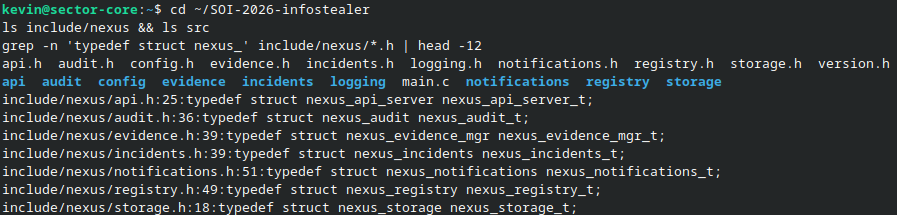
\includegraphics[width=0.82\textwidth,height=3.5cm,keepaspectratio]{images/etapa01_estructura_modulos.png}
    \caption{Árbol de directorios y organización de submódulos en el código fuente de \texttt{nexusd}.}
    \label{fig:etapa01_arbol}
\end{figure}

% ==============================================================================
% ETAPA 02 — PERSISTENCIA
% ==============================================================================
\section{Etapa 02 — Persistencia de Datos con SQLite}

Toda la información del sector se modela de manera relacional y se almacena en SQLite, garantizando persistencia durable en el archivo de base de datos ubicado canónicamente en \texttt{/var/lib/nexus/nexus.db}.

\subsection{Modelo de Datos y Esquema DDL}

El esquema contempla las entidades requeridas con restricciones estrictas de integridad referencial, tipos y dominios:

\begin{table}[H]
    \centering
    \footnotesize
    \caption{Definición de entidades y atributos requeridos para la base de datos de \texttt{nexusd}.}
    \label{tab:entidades_sqlite}
    \begin{tabularx}{\textwidth}{p{1.7cm} >{\raggedright\arraybackslash}p{3.8cm} X}
        \toprule
        \rowcolor{tableheader}
        \textbf{Entidad} & \textbf{Atributos Principales} & \textbf{Restricciones / Reglas de Validación} \\
        \midrule
        \textbf{Unidad} & \texttt{id}, \texttt{designation}, \texttt{model}, \texttt{status}, \texttt{sector}, \texttt{created\_at} & \texttt{designation} identificador alfanumérico textual. \texttt{status} restringido a valores válidos: \textit{active}, \textit{standby}, \textit{maintenance}, \textit{decommissioned}. \\
        \rowcolor{rowalt}
        \textbf{Operador} & \texttt{id}, \texttt{name}, \texttt{clearance\_level}, \texttt{active}, \texttt{created\_at} & \texttt{clearance\_level} entero no negativo ($\ge 0$). \texttt{active} valor booleano binario (\texttt{0} o \texttt{1}). \\
        \textbf{Incidente} & \texttt{id}, \texttt{unit\_id}, \texttt{operator\_id}, \texttt{severity}, \texttt{description}, \texttt{status}, \texttt{created\_at}, \texttt{updated\_at} & Claves foráneas hacia \texttt{units} y \texttt{operators}. Dominios restringidos de \texttt{severity} y \texttt{status}. \\
        \rowcolor{rowalt}
        \textbf{Evidencia} & \texttt{id}, \texttt{incident\_id}, \texttt{filename}, \texttt{checksum}, \texttt{uploaded\_at} & Clave foránea referencial a incidente. \texttt{checksum} SHA-256 en codificación hexadecimal (64 caracteres). \\
        \textbf{Auditoría} & \texttt{id}, \texttt{actor}, \texttt{action}, \texttt{resource}, \texttt{result}, \texttt{timestamp} & Registro append-only inmutable de eventos transaccionales del sistema. \\
        \bottomrule
    \end{tabularx}
\end{table}

\begin{terminalbox}{sqlite_schema.sql}
CREATE TABLE units ( id INTEGER PRIMARY KEY AUTOINCREMENT, designation TEXT NOT NULL, model TEXT NOT NULL, status TEXT NOT NULL, sector TEXT NOT NULL, created_at INTEGER NOT NULL, CHECK (status IN ('active','standby','maintenance','decommissioned')));
CREATE TABLE operators ( id INTEGER PRIMARY KEY AUTOINCREMENT, name TEXT NOT NULL, clearance_level INTEGER NOT NULL, active INTEGER NOT NULL DEFAULT 1, created_at INTEGER NOT NULL, CHECK (clearance_level >= 0), CHECK (active IN (0, 1)));
CREATE TABLE incidents ( id INTEGER PRIMARY KEY AUTOINCREMENT, unit_id INTEGER NOT NULL, operator_id INTEGER NOT NULL, severity TEXT NOT NULL, description TEXT NOT NULL, status TEXT NOT NULL, created_at INTEGER NOT NULL, updated_at INTEGER NOT NULL, CHECK (severity IN ('low','medium','high','critical')), CHECK (status IN ('open','investigating','resolved','closed')), FOREIGN KEY (unit_id) REFERENCES units(id), FOREIGN KEY (operator_id) REFERENCES operators(id));
CREATE TABLE evidence ( id INTEGER PRIMARY KEY AUTOINCREMENT, incident_id INTEGER NOT NULL, filename TEXT NOT NULL, checksum TEXT NOT NULL, uploaded_at INTEGER NOT NULL, FOREIGN KEY (incident_id) REFERENCES incidents(id));
CREATE TABLE audit_events ( id INTEGER PRIMARY KEY AUTOINCREMENT, actor TEXT NOT NULL, action TEXT NOT NULL, resource TEXT NOT NULL, result TEXT NOT NULL, timestamp INTEGER NOT NULL);
\end{terminalbox}

\subsection{Fundamentación Teórica y Preguntas de Investigación}

\begin{pregunta}{¿Qué significa que SQLite sea una base embebida? ¿Dónde corre realmente?}
    \textbf{Respuesta:} A diferencia de un Sistema de Gestión de Bases de Datos (RDBMS) cliente-servidor tradicional (como PostgreSQL o MariaDB), SQLite no es un proceso daemon independiente ni escucha en un socket de red. SQLite es una biblioteca compilada estática o dinámicamente (\texttt{libsqlite3}) que se enlaza y se ejecuta directamente en el \textbf{mismo espacio de direcciones de memoria (user-space)} del proceso \texttt{nexusd}.
    
    La base de datos corre físicamente dentro del proceso que la invoca. Cuando \texttt{nexusd} ejecuta una consulta SQL, no se produce ninguna comunicación inter-proceso (IPC) ni intercambio de paquetes de red: son llamadas a funciones directas en lenguaje C que interactúan con el kernel mediante llamadas al sistema de archivos (\texttt{open}, \texttt{read}, \texttt{write}, \texttt{fcntl}, \texttt{fsync}) sobre un único archivo regular en disco (\texttt{nexus.db}).
\end{pregunta}

\begin{pregunta}{¿Qué pasa si dos partes del programa escriben al mismo tiempo?}
    \textbf{Respuesta:} SQLite gestiona la concurrencia a nivel de archivo utilizando bloqueos del sistema de archivos (\textit{POSIX file advisory locks} o locks nativos de SO). En el modo tradicional de \textit{rollback journal}, SQLite admite múltiples lectores concurrentes pero únicamente \textbf{un único escritor a la vez} (bloqueo exclusivo sobre la base completa).
    
    Si una parte del programa intenta iniciar una transacción de escritura mientras otra ya posee el bloqueo exclusivo, SQLite devolverá de forma inmediata el código de error \texttt{SQLITE\_BUSY}. Para evitar fallos abruptos, se configura la llamada \texttt{sqlite3\_busy\_timeout()}, la cual instruye a la biblioteca a reintentar la operación durante un intervalo configurable (ej. 5000 ms) antes de declinar la transacción. Adicionalmente, al activar el modo \textbf{WAL} (\textit{Write-Ahead Logging}, \texttt{PRAGMA journal\_mode=WAL;}), los lectores no bloquean a los escritores y el escritor no bloquea a los lectores, optimizando sustancialmente el rendimiento concurrente.
\end{pregunta}

\begin{pregunta}{¿Qué es una transacción y cuándo conviene usar una?}
    \textbf{Respuesta:} Una transacción es una unidad lógica de trabajo compuesta por una o más sentencias SQL ejecutadas de forma indivisible bajo el principio de garantías \textbf{ACID}:
    \begin{itemize}[leftmargin=*]
        \item \textbf{Atomicidad:} O se completan todas las operaciones con éxito (\texttt{COMMIT}) o el sistema revierte cualquier cambio intermedio (\texttt{ROLLBACK}), evitando estados corruptos parciales.
        \item \textbf{Consistencia:} La base de datos transita de un estado válido a otro respetando todas las restricciones de integridad (claves foráneas, unicidad, checks).
        \item \textbf{Aislamiento:} Las transacciones concurrentes operan sin interferir entre sí.
        \item \textbf{Durabilidad:} Una vez confirmado el commit, las modificaciones persisten incluso ante fallas de alimentación eléctrica o cierres abruptos del sistema operativo.
    \end{itemize}
    Conviene utilizar transacciones explícitas (\texttt{BEGIN TRANSACTION} ... \texttt{COMMIT}) siempre que se realicen inserciones o modificaciones multietapa vinculadas (por ejemplo: insertar un incidente e inmediatamente registrar su correspondiente evento en la tabla de auditoría), y también para agrupar inserciones masivas, reduciendo la cantidad de llamadas costosas a sincronización en disco (\texttt{fsync}).
\end{pregunta}

\begin{pregunta}{¿Qué diferencia hay entre que una escritura "retorne" y que esté efectivamente en disco?}
    \textbf{Respuesta:} Cuando un proceso invoca la llamada al sistema \texttt{write(2)}, los datos son transferidos desde el buffer de memoria de usuario hacia la memoria intermedia del kernel del sistema operativo (\textbf{Page Cache}). Para optimizar el rendimiento de entrada/salida (I/O), la llamada al sistema retorna de inmediato al espacio de usuario una vez que los datos residen en la Page Cache (quedando marcadas como \textit{dirty pages}).
    
    Sin embargo, que la escritura haya "retornado" \textbf{no significa que esté grabada físicamente en el plato magnético o celda de memoria flash del disco}. Las páginas sucias permanecen en memoria RAM volátil hasta que los hilos del kernel (\texttt{flusher/pdflush}) las vuelcan al disco, o hasta que el proceso emite explícitamente una llamada sincrónica como \textbf{\texttt{fsync(2)}} o \textbf{\texttt{fdatasync(2)}}. Si ocurre un corte de energía mientras los datos están sólo en la Page Cache, la información se pierde irremediablemente. SQLite asegura la durabilidad emitiendo \texttt{fsync} durante el cierre de cada transacción confirmada.
\end{pregunta}

\begin{pregunta}{¿Qué puede salir mal si el proceso termina en medio de una escritura?}
    \textbf{Respuesta:} Si un proceso es terminado de forma abrupta (por ejemplo por una señal \texttt{SIGKILL} o corte de energía) mientras escribe sin una capa transaccional robusta, el archivo de datos puede quedar en un estado parcialmente modificado: punteros de árboles B truncados, sectores incompletos o registros a medio grabar, provocando la corrupción irreversible de la base de datos.
    
    SQLite previene esta catástrofe mediante su mecanismo de registro atómico:
    \begin{enumerate}[leftmargin=*]
        \item En modo \textit{Rollback Journal}: Antes de modificar cualquier página de la base de datos, SQLite crea un archivo auxiliar (\texttt{.db-journal}) donde copia las páginas originales intactas y hace un \texttt{fsync}. Solo después modifica la base. Si el proceso cae en el medio, al siguiente inicio SQLite detecta el journal pendiente y restablece las páginas originales (\textit{hot journal rollback}).
        \item En modo \textit{WAL}: Las escrituras se anexan al archivo de log (\texttt{.db-wal}). Si el proceso finaliza a mitad de una transacción no confirmada, los cambios incompletos son simplemente descartados durante la recuperación, garantizando que el archivo principal (\texttt{.db}) nunca se corrompa.
    \end{enumerate}
\end{pregunta}

\subsection{Verificación Experimental del Esquema y Persistencia en SQLite}

En la Figura~\ref{fig:etapa02_persistencia} se documenta la inspección directa del archivo de base de datos relacional ubicado en \texttt{/var/lib/nexus/}\allowbreak\texttt{nexus.db} utilizando la interfaz de línea de comandos \texttt{sqlite3}. Se constata la correcta instanciación de las tablas de unidades, operadores, incidentes, evidencias y eventos de auditoría, verificando la presencia de claves primarias autoincrementales, restricciones foráneas y dominios de validación (\texttt{CHECK}).

\begin{figure}[H]
    \centering
    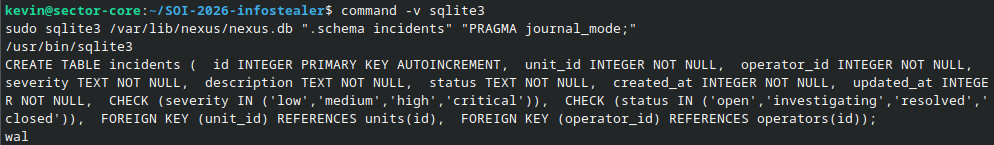
\includegraphics[width=0.82\textwidth,height=3.5cm,keepaspectratio]{images/etapa02_persistencia_sqlite.png}
    \caption{Inspección del esquema relacional y estado de las tablas en SQLite mediante la CLI \texttt{sqlite3}.}
    \label{fig:etapa02_persistencia}
\end{figure}

% ==============================================================================
% ETAPA 03 — LA API DEL SECTOR
% ==============================================================================
\section{Etapa 03 — La API HTTP del Sector}

El daemon \texttt{nexusd} expone una interfaz de programación de aplicaciones (API) REST versionada bajo el prefijo canónico \texttt{/api/v1/}, además de un punto de diagnóstico de salud en la raíz (\texttt{/health}). La comunicación utiliza estrictamente cargas útiles codificadas en formato \textbf{JSON} (\texttt{application/json}), con códigos de estado HTTP semánticos y esquemas de error descriptivos.

\subsection{Matriz de Endpoints y Contratos de Servicio}

\begin{table}[H]
    \centering
    \footnotesize
    \caption{Catálogo de operaciones expuestas por la API de \texttt{nexusd}.}
    \label{tab:api_endpoints}
    \begin{tabularx}{\textwidth}{llXl}
        \toprule
        \rowcolor{tableheader}
        \textbf{Método} & \textbf{Ruta / Endpoint} & \textbf{Propósito / Operación} & \textbf{Códigos HTTP} \\
        \midrule
        \texttt{GET} & \texttt{/health} & Verificación del estado de \texttt{nexusd} y conectividad a SQLite. & \texttt{200}, \texttt{503} \\
        \rowcolor{rowalt}
        \texttt{GET} & \texttt{/api/v1/units} & Listado completo de unidades operativas del sector. & \texttt{200} \\
        \texttt{POST} & \texttt{/api/v1/units} & Alta de una nueva unidad operativa. & \texttt{201}, \texttt{400} \\
        \rowcolor{rowalt}
        \texttt{GET} & \texttt{/api/v1/operators} & Listado de operadores registrados en el sistema. & \texttt{200} \\
        \texttt{POST} & \texttt{/api/v1/operators} & Alta de un nuevo operador en el registro. & \texttt{201}, \texttt{400} \\
        \rowcolor{rowalt}
        \texttt{GET} & \texttt{/api/v1/incidents} & Listado de incidentes registrados en el sector. & \texttt{200} \\
        \texttt{GET} & \texttt{/api/v1/incidents/\{id\}} & Consulta en detalle de un incidente específico. & \texttt{200}, \texttt{404} \\
        \rowcolor{rowalt}
        \texttt{POST} & \texttt{/api/v1/incidents} & Registro y asignación de un nuevo incidente. & \texttt{201}, \texttt{400} \\
        \texttt{PATCH} & \texttt{/api/v1/incidents/\{id\}} & Actualización del estado de un incidente. & \texttt{200}, \texttt{400}, \texttt{404}, \texttt{422} \\
        \rowcolor{rowalt}
        \texttt{GET} & \texttt{/api/v1/incidents/\{id\}/evidence} & Listado de evidencias asociadas a un incidente. & \texttt{200}, \texttt{404} \\
        \texttt{POST} & \texttt{/api/v1/incidents/\{id\}/evidence} & Alta de nueva evidencia digital en un incidente. & \texttt{201}, \texttt{400}, \texttt{404} \\
        \rowcolor{rowalt}
        \texttt{GET} & \texttt{/api/v1/audit} & Consulta del registro inmutable de eventos de auditoría. & \texttt{200} \\
        \bottomrule
    \end{tabularx}
\end{table}

\begin{notabox}[Aislamiento de Red del Demonio]
    En este capítulo, el socket TCP del daemon escucha exclusivamente en la dirección de bucle local (\textbf{\texttt{127.0.0.1:8080}}). No se expone directamente a interfaces públicas; en el Capítulo 3 se incorporará el proxy inverso Nginx como único punto de entrada perimetral.
\end{notabox}

\subsection{Fundamentación Teórica y Preguntas de Investigación}

\begin{pregunta}{¿Qué códigos HTTP corresponden a: recurso creado, dato inválido, recurso inexistente y error interno?}
    \textbf{Respuesta:}
    \begin{itemize}[leftmargin=*]
        \item \textbf{Recurso Creado -- \texttt{201 Created}:} Confirma que la petición fue procesada exitosamente y derivó en la instanciación persistente de un nuevo recurso en la base de datos (generalmente devolviendo la entidad creada y su nuevo identificador \texttt{id}).
        \item \textbf{Dato Inválido / Malformado -- \texttt{400 Bad Request}:} Indica que el servidor no puede procesar la solicitud debido a un error del cliente: sintaxis JSON inválida, omisión de campos requeridos (ej. falta \texttt{designation} en una unidad), o tipos de datos incompatibles.
        \item \textbf{Recurso Inexistente -- \texttt{404 Not Found}:} El endpoint o identificador numérico solicitado no existe en la base de datos (por ejemplo, intentar modificar mediante \texttt{PATCH /api/v1/incidents/9999} un incidente que no está registrado).
        \item \textbf{Error Interno -- \texttt{500 Internal Server Error}:} Señaliza una falla imprevista en el espacio del servidor: fallo al acceder al archivo SQLite por permisos corruptos, agotamiento de descriptores de archivos, o error inesperado de I/O.
        \item \textbf{Entidad No Procesable -- \texttt{422 Unprocessable Entity}:} El JSON es sintácticamente válido pero la transición de estado solicitada no está permitida entre los estados del ciclo de vida del incidente (error \texttt{"invalid\_transition"}).
    \end{itemize}
\end{pregunta}

\begin{pregunta}{¿Por qué PATCH y no POST para cambiar el estado de un incidente?}
    \textbf{Respuesta:} De acuerdo con los estándares de arquitectura REST y las especificaciones RFC 7231 y RFC 5789:
    \begin{itemize}[leftmargin=*]
        \item \textbf{\texttt{POST}} está concebido semánticamente para la creación de un nuevo recurso subordinado en una colección, o para invocar operaciones no idempotentes.
        \item \textbf{\texttt{PUT}} está destinado al reemplazo completo de un recurso preexistente, obligando al cliente a reenviar el cuerpo íntegro con todos sus atributos.
        \item \textbf{\texttt{PATCH}} fue diseñado formalmente (RFC 5789) para aplicar una \textbf{modificación parcial} sobre un recurso existente.
    \end{itemize}
    Dado que una transición de incidente únicamente requiere actualizar atributos puntuales (como \texttt{status = "investigating"} o \texttt{severity = "high"}) preservando inalterados el resto de los metadatos (\texttt{description}, \texttt{unit\_id}, \texttt{created\_at}), el verbo HTTP adecuado y semánticamente correcto es \textbf{\texttt{PATCH}}.
\end{pregunta}

\begin{pregunta}{¿Para qué sirve versionar una API bajo /api/v1/?}
    \textbf{Respuesta:} El versionado explícito en la URI garantiza el principio de \textbf{estabilidad de contratos} e interoperabilidad evolutiva en sistemas distribuidos. Permite que el equipo de desarrollo introduzca cambios disruptivos (\textit{breaking changes}) en la estructura de datos, formatos o autenticación creando un nuevo conjunto de rutas bajo \texttt{/api/v2/}, sin romper de manera destructiva los clientes o scripts de campo antiguos que continúen consumiendo la interfaz bajo \texttt{/api/v1/}. Otorga un ciclo de deprecación ordenado y seguro en entornos de producción.
\end{pregunta}

\subsection{Verificación Experimental y Evidencia de Funcionamiento}

Para constatar el correcto funcionamiento de la interfaz de red y la capa de almacenamiento relacional, se ejecutó un conjunto exhaustivo de pruebas directamente contra la API de \texttt{nexusd} mediante peticiones HTTP (\texttt{curl}), verificando el formato de salida JSON y la consistencia transaccional.

En primer lugar, se validó la capacidad de listar las entidades existentes y consultar el detalle pormenorizado de un incidente específico, así como la transición formal de estados a través de la ruta oficial de actualización mediante el verbo \texttt{PATCH} (Figura~\ref{fig:etapa03_consultas_transicion}).

\begin{figure}[H]
    \centering
    \begin{subfigure}[b]{0.48\textwidth}
        \centering
        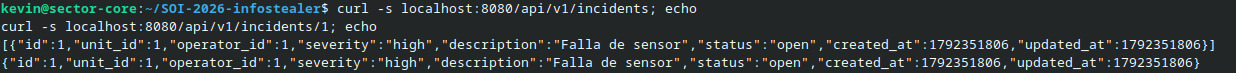
\includegraphics[width=\textwidth,height=3.0cm,keepaspectratio]{images/etapa03_prueba_a_listar.jpg}
        \caption{Prueba A: Listado y consulta en detalle de incidentes registrados vía \texttt{GET /api/v1/incidents}.}
        \label{fig:etapa03_prueba_a}
    \end{subfigure}
    \hfill
    \begin{subfigure}[b]{0.48\textwidth}
        \centering
        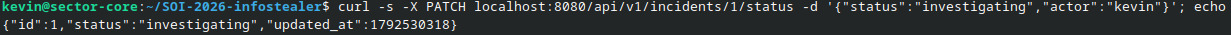
\includegraphics[width=\textwidth,height=3.0cm,keepaspectratio]{images/etapa03_prueba_b_cambiar_estado.jpg}
        \caption{Prueba B: Transición de estado a través de la ruta oficial con \texttt{PATCH /api/v1/incidents/\{id\}/status}.}
        \label{fig:etapa03_prueba_b}
    \end{subfigure}
    \caption{Verificación operativa de la API de \texttt{nexusd}: consultas estructuradas en JSON y transición atómica de estados.}
    \label{fig:etapa03_consultas_transicion}
\end{figure}

Posteriormente, se verificó la gestión de evidencias digitales asociadas a incidentes, corroborando que el sistema exige y valida la integridad criptográfica mediante el hash SHA-256 del archivo. Asimismo, se comprobó que cada operación de alta o modificación genera de forma síncrona y transaccional una entrada en la tabla inmutable de auditoría (\texttt{audit\_events}), registrando el actor, la acción, el recurso impactado y la marca temporal (Figura~\ref{fig:etapa03_evidencia_auditoria}).

\begin{figure}[H]
    \centering
    \begin{subfigure}[b]{0.48\textwidth}
        \centering
        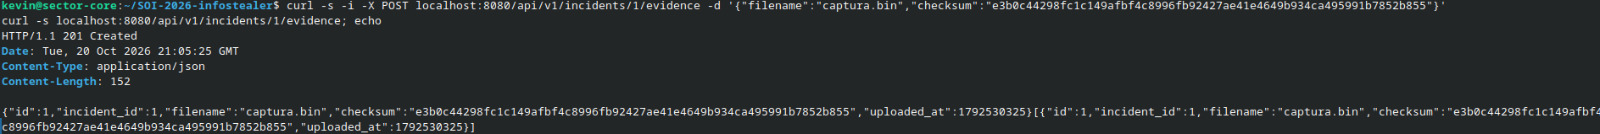
\includegraphics[width=\textwidth,height=3.0cm,keepaspectratio]{images/etapa03_prueba_c_evidencia.jpg}
        \caption{Prueba C: Alta de evidencia digital con verificación estricta de checksum SHA-256 y consulta posterior.}
        \label{fig:etapa03_prueba_c}
    \end{subfigure}
    \hfill
    \begin{subfigure}[b]{0.48\textwidth}
        \centering
        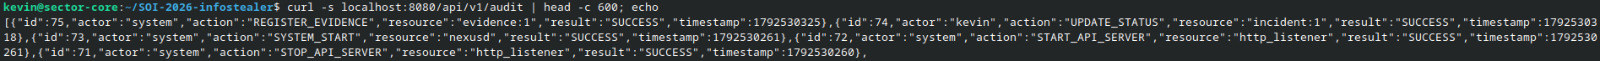
\includegraphics[width=\textwidth,height=3.0cm,keepaspectratio]{images/etapa03_prueba_d_auditoria.jpg}
        \caption{Prueba D: Registro inmutable de eventos en la tabla de auditoría ante cada acción relevante.}
        \label{fig:etapa03_prueba_d}
    \end{subfigure}
    \caption{Gestión de evidencias digitales y trazabilidad transaccional en la base de datos SQLite.}
    \label{fig:etapa03_evidencia_auditoria}
\end{figure}

Por último, se puso a prueba la robustez del servidor ante casos de error límite: envío de un checksum con longitud o caracteres no hexadecimales, consulta de un identificador de incidente inexistente y envío de identificadores con tipos incompatibles. Como se observa en la Figura~\ref{fig:etapa03_errores}, la API rechaza consistentemente las anomalías con códigos semánticos (\texttt{400 Bad Request} y \texttt{404 Not Found}), emitiendo un objeto JSON explicativo y sin degradar la estabilidad del daemon.

\begin{figure}[H]
    \centering
    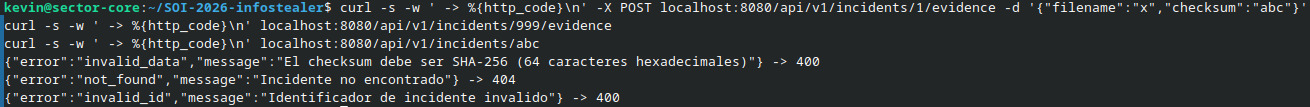
\includegraphics[width=0.85\textwidth,height=3.4cm,keepaspectratio]{images/etapa03_prueba_e_errores.jpg}
    \caption{Prueba E: Validación de semántica y códigos de error HTTP ante checksum inválido, incidente inexistente e ID malformado.}
    \label{fig:etapa03_errores}
\end{figure}

% ==============================================================================
% ETAPA 04 — CONFIGURACIÓN EXTERNA
% ==============================================================================
\section{Etapa 04 — Configuración Externa}

Siguiendo las mejores prácticas de ingeniería de software de sistemas (los Doce Factores para aplicaciones y el estándar FHS), el daemon \texttt{nexusd} no codifica (\textit{hardcodea}) ninguna ruta, puerto o credencial en su código fuente binario. Todas las variables operativas se leen en tiempo de inicio desde un archivo de configuración externo estandarizado: \textbf{\texttt{/etc/nexus/nexus.conf}}.

\subsection{Estructura del Archivo de Configuración}

\begin{terminalbox}{/etc/nexus/nexus.conf}
[server]
listen_address = 127.0.0.1
listen_port = 8080

[database]
database_path = /var/lib/nexus/nexus.db

[storage]
evidence_path = /var/lib/nexus/evidence

[logging]
level = info
\end{terminalbox}

\subsection{Fundamentación Teórica y Preguntas de Investigación}

\begin{pregunta}{¿Qué debería hacer el programa si el archivo no existe? ¿Y si existe pero tiene una línea inválida?}
    \textbf{Respuesta:} La implementación de \texttt{nexusd} sigue una política estricta de \textbf{Fallo Temprano (\textit{Fail-Fast})}:
    \begin{itemize}[leftmargin=*]
        \item \textbf{Archivo Inexistente:} El programa emite un mensaje de error explícito en \texttt{stderr} indicando la ruta del archivo ausente, se niega a iniciar la ejecución y finaliza de inmediato con código de salida \texttt{1}, alertando al administrador sobre la omisión de la configuración.
        \item \textbf{Línea, Sección o Valor Inválido:} El analizador sintáctico no tolera ambigüedades. Ante cualquier clave desconocida, sintaxis rota o valor fuera de dominio (ej. un nivel de log no reconocido o un puerto inválido), el daemon imprime el error detallando el archivo y el número de línea offending, aborta el arranque y termina con código de salida \texttt{1}.
    \end{itemize}
\end{pregunta}

\begin{pregunta}{¿Conviene arrancar con valores por defecto o negarse a arrancar?}
    \textbf{Respuesta:} En un servicio crítico del sistema operativo como \texttt{nexusd}, la práctica profesional y determinista es \textbf{negarse rotundamente a arrancar} ante cualquier anomalía:
    \begin{itemize}[leftmargin=*]
        \item \textbf{Riesgo de los valores por defecto:} Asumir valores predeterminados de forma silenciosa puede provocar que el servicio intente enlazarse a interfaces no deseadas, intente escribir en rutas sin permisos o degrade el nivel de auditoría sin el conocimiento explícito del administrador de sistemas.
        \item \textbf{Determinismo estricto:} Por diseño, el daemon no recurre a valores por defecto silenciosos. Cada parámetro operacional debe estar explícitamente configurado y validado en \texttt{/etc/nexus/nexus.conf}. Si el archivo no existe o contiene anomalías, el servicio aborta de inmediato con código \texttt{1}, garantizando que sólo opere bajo un estado enteramente consistente y verificado.
    \end{itemize}
\end{pregunta}

\begin{pregunta}{¿Qué permisos debería tener un archivo de configuración de un servicio del sistema?}
    \textbf{Respuesta:} Aplicando el Principio de Mínimo Privilegio (PoLP):
    \begin{itemize}[leftmargin=*]
        \item Propietario usuario: \texttt{root} (para evitar que un proceso comprometido pueda reescribir su propia configuración).
        \item Grupo propietario: \texttt{nexus} (el grupo del servicio).
        \item Permisos octales: \textbf{\texttt{0640}} (\texttt{rw-r-----}).
    \end{itemize}
    Esto garantiza que el administrador (\texttt{root}) pueda leer y modificar el archivo, el demonio (\texttt{nexus}) pueda leerlo durante el inicio o recarga, y cualquier otro usuario o atacante sin privilegios en el sistema tenga \textbf{acceso totalmente denegado} (\texttt{---}). Si el archivo contiene credenciales sensibles o secretos criptográficos, los permisos deben ser aún más restrictivos (\textbf{\texttt{0600}} exclusivo para el usuario que ejecuta el proceso).
\end{pregunta}

\begin{pregunta}{¿Por qué /etc y no el directorio del programa?}
    \textbf{Respuesta:} Esta convención responde al estándar \textbf{FHS (\textit{Filesystem Hierarchy Standard})} adoptado por todas las distribuciones GNU/Linux:
    \begin{itemize}[leftmargin=*]
        \item \textbf{\texttt{/etc}} es el directorio del sistema destinado específicamente a archivos de configuración estática del host. Permite centralizar la administración, respaldar las configuraciones de todas las aplicaciones en un solo punto y preservarlas ante actualizaciones del binario.
        \item Los directorios donde residen los binarios ejecutables (\texttt{/usr/bin}, \texttt{/usr/local/bin}) están diseñados para ser de \textbf{sólo lectura} (\textit{read-only}) e incluso pueden montarse compartidos en red. Colocar archivos de configuración junto al ejecutable viola la separación funcional entre código binario inmutable y estado/configuración local del nodo.
    \end{itemize}
\end{pregunta}

\begin{pregunta}{¿Qué parte de la configuración tiene sentido poder recargar sin reiniciar el proceso?}
    \textbf{Respuesta:}
    \begin{itemize}[leftmargin=*]
        \item \textbf{Recargable dinámicamente:} Directivas que alteran el comportamiento lógico sin destruir descriptores de red ni estructuras de bajo nivel. Ejemplos: \texttt{log\_level} (cambiar de \texttt{info} a \texttt{debug} para diagnosticar un incidente en caliente), listas de control de acceso, o políticas de timeouts.
        \item \textbf{No recargable en caliente (requiere reinicio completo):} Parámetros ligados a recursos del sistema que implican destrucción y recreación de sockets o manejadores principales, tales como \texttt{listen\_address} y \texttt{listen\_port} (requieren cerrar el socket pasivo, desasociar la interfaz, emitir nuevo \texttt{bind(2)} y \texttt{listen(2)}) o la ruta de la base de datos (\texttt{database\_path}), que obligaría a cerrar el manejador SQLite y drenar abruptamente transacciones en curso.
    \end{itemize}
\end{pregunta}

\subsection{Verificación Experimental de la Configuración Externa}

Se constató empíricamente la robustez del manejo de configuración externa en \texttt{nexusd}. En la Figura~\ref{fig:etapa04_config}(a) se documenta el esquema estricto de permisos sobre \texttt{/etc/nexus/nexus.conf} (\texttt{0640}, \texttt{root:nexus}), comprobando que el usuario del servicio lee el archivo sin trabas mientras que un usuario sin privilegios recibe \textit{Permission denied}. En la Figura~\ref{fig:etapa04_config}(b) se valida experimentalmente el comportamiento \textbf{Fail-Fast}: al intentar arrancar el daemon con una ruta inexistente (\texttt{/tmp/no-existe.conf}) o con una directiva inválida (\texttt{level = ruidoso}), el binario emite un mensaje de error descriptivo en \texttt{stderr} y aborta de inmediato con código de salida \texttt{1}, impidiendo la ejecución en estados corrompidos.

\begin{figure}[H]
    \centering
    \begin{subfigure}[b]{0.48\textwidth}
        \centering
        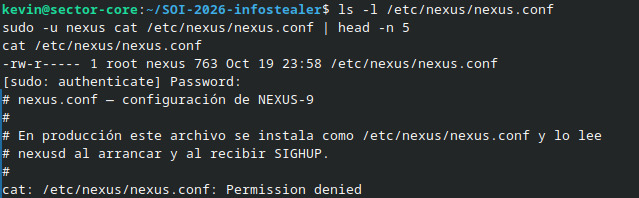
\includegraphics[width=\textwidth,height=3.0cm,keepaspectratio]{images/etapa04_config_nexus.jpg}
        \caption{Permisos \texttt{0640} (\texttt{root:nexus}): lectura por \texttt{nexus} y denegada a terceros.}
        \label{fig:etapa04_conf_file}
    \end{subfigure}
    \hfill
    \begin{subfigure}[b]{0.48\textwidth}
        \centering
        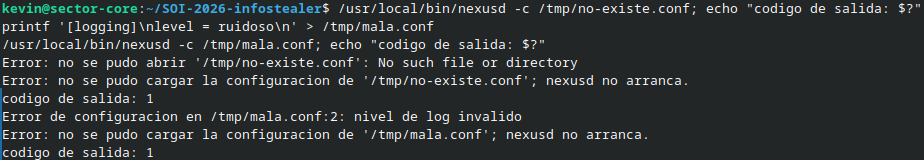
\includegraphics[width=\textwidth,height=3.0cm,keepaspectratio]{images/etapa04_configuracion_conf.png}
        \caption{Validación Fail-Fast: aborto (código 1) ante archivo inexistente y valor inválido.}
        \label{fig:etapa04_conf_run}
    \end{subfigure}
    \caption{Gestión de configuración externa: aislamiento de privilegios y tolerancia a fallos (\textit{fail-fast}).}
    \label{fig:etapa04_config}
\end{figure}

% ==============================================================================
% ETAPA 05 — SEÑALES Y CICLO DE VIDA
% ==============================================================================
\section{Etapa 05 — Señales y Ciclo de Vida del Proceso}

Un proceso de sistema no decide cuándo finaliza ni cuándo su entorno cambia: es el sistema operativo quien se lo notifica a través de \textbf{señales POSIX}. El daemon \texttt{nexusd} implementa un manejador asincrónico estructurado para gestionar de forma determinista el apagado controlado y la recarga en caliente.

\subsection{Matriz de Señales Soportadas}

\begin{table}[H]
    \centering
    \footnotesize
    \caption{Tratamiento y comportamiento del manejador de señales en \texttt{nexusd}.}
    \label{tab:senales}
    \begin{tabularx}{\textwidth}{llX}
        \toprule
        \rowcolor{tableheader}
        \textbf{Señal POSIX} & \textbf{Disparador / Origen} & \textbf{Acción Ejecutada por \texttt{nexusd}} \\
        \midrule
        \textbf{\texttt{SIGTERM}} & Emitida por \texttt{systemd} al ejecutar \texttt{systemctl stop nexus}. & Cierre ordenado (\textit{graceful shutdown}): se detiene el bucle de eventos, se completan transacciones en curso, se cierra la base SQLite (\texttt{sqlite3\_close\_v2}) y se liberan descriptores de red. \\
        \rowcolor{rowalt}
        \textbf{\texttt{SIGINT}} & Teclado interactivo (\texttt{Ctrl+C}) en modo desarrollo/pruebas. & Mismo procedimiento que \texttt{SIGTERM}: apagado controlado y salida con código \texttt{0}. \\
        \textbf{\texttt{SIGHUP}} & Emitida por \texttt{systemctl reload nexus} o \texttt{kill -HUP <PID>}. & Recarga en caliente: relectura del archivo \texttt{/etc/nexus/nexus.conf} actualizando el nivel de log (\texttt{log\_level}) sin reiniciar el proceso ni desconectar clientes. \\
        \bottomrule
    \end{tabularx}
\end{table}

\subsection{Fundamentación Teórica y Preguntas de Investigación}

\begin{pregunta}{¿Qué operaciones son seguras dentro de un manejador de señales? Investiguen signal-safety(7).}
    \textbf{Respuesta:} Según la especificación POSIX y la página de manual \texttt{signal-safety(7)}, únicamente son seguras aquellas funciones declaradas como \textbf{\textit{Async-Signal-Safe}} (reentrantes o que no pueden ser interrumpidas en un estado inconsistente).
    
    Un manejador de señales se ejecuta de manera asíncrona, interrumpiendo el flujo normal del hilo en cualquier instrucción máquina. Si el hilo principal se encontraba a mitad de una llamada a \texttt{malloc()} (modificando la lista enlazada del heap del proceso) o en \texttt{printf()} (adquiriendo el lock del buffer de I/O de \texttt{stdout}), e invoca dentro del manejador a \texttt{malloc} o \texttt{printf}, se produce una \textbf{condición de carrera destructiva o un bloqueo mutuo (\textit{deadlock})}. Por ende, funciones de \texttt{stdio.h}, asignación dinámica de memoria (\texttt{malloc}/\texttt{free}) y operaciones de SQLite \textbf{están estrictamente prohibidas dentro de un signal handler}. Solo llamadas al sistema de bajo nivel como \texttt{write(2)}, \texttt{sigaction(2)} o la asignación a tipos atómicos son seguras.
\end{pregunta}

\begin{pregunta}{¿Por qué un manejador suele limitarse a levantar una bandera en lugar de hacer el trabajo?}
    \textbf{Respuesta:} Por la restricción intrínseca de reentrancia explicada en \texttt{signal-safety(7)}. Para no comprometer la estabilidad del proceso, la arquitectura estándar de daemons UNIX adopta el patrón de \textbf{bandera atómica}:
    \begin{itemize}[leftmargin=*]
        \item El manejador de señal se limita a escribir en una variable de control declarada como \textbf{\texttt{volatile sig\_atomic\_t g\_stop\_requested = 1;}} (o usando primitivas atómicas de C11/C17). Esta operación es atómica en hardware y garantizada como async-signal-safe.
        \item El bucle principal de la aplicación (\textit{event loop}), que corre en el contexto normal de ejecución del hilo, chequea periódicamente dicha bandera. Cuando la detecta en alto, es el hilo principal quien procede de forma síncrona y segura a cerrar conexiones, liberar memoria con \texttt{free()} y cerrar SQLite con \texttt{sqlite3\_close\_v2()}.
    \end{itemize}
\end{pregunta}

\begin{pregunta}{¿Qué pasa con una escritura a la base si el proceso muere en el medio?}
    \textbf{Respuesta:} Si el proceso es alcanzado por una señal no capturable como \texttt{SIGKILL} (\texttt{kill -9}) o un fallo catastrófico de hardware durante una transacción no confirmada, el proceso desaparece inmediatamente sin ejecutar código de limpieza.
    
    Sin embargo, gracias al diseño transaccional y los mecanismos de \textit{journaling} (o \textit{WAL}) de SQLite:
    \begin{itemize}[leftmargin=*]
        \item Las escrituras a medio completar quedan confinadas en el archivo temporal o el log de pre-escritura.
        \item El archivo maestro \texttt{nexus.db} conserva intactas las páginas previas.
        \item En el siguiente arranque del servicio, el subsistema de SQLite realiza automáticamente la recuperación hacia atrás (\textit{rollback recovery}), restaurando la base al último estado consistente confirmado. Estos mecanismos protegen la integridad de la base ante la gran mayoría de escenarios de fallo.
    \end{itemize}
\end{pregunta}

\begin{pregunta}{¿Por qué SIGHUP se usa históricamente para recargar configuración?}
    \textbf{Respuesta:} Históricamente, en los inicios de los sistemas UNIX conectados a terminales tele-tipo mediante módems telefónicos, la señal \textbf{\texttt{SIGHUP} (\textit{Signal Hangup})} era generada por el controlador serie de la tty para avisar a los procesos de la sesión que la línea telefónica se había cortado físicamente (\textit{hang up}).
    
    Dado que un daemon de sistema se desasocia completamente de su terminal controladora al nacer, la señal \texttt{SIGHUP} pierde su propósito original de desconexión. Por esta razón, la comunidad UNIX adoptó por convención universal reutilizar \texttt{SIGHUP} como una señal de notificación de propósito general: al recibirla, el daemon interpreta que debe releer sus archivos de configuración en \texttt{/etc} y actualizar su estado interno sin interrumpir sus servicios ni dar de baja a sus conexiones activas.
\end{pregunta}

\subsection{Verificación Experimental del Manejo de Señales POSIX}

Para certificar que el ciclo de vida del proceso se gestiona de forma determinista y conforme al estándar POSIX, se sometió a \texttt{nexusd} a pruebas de terminación y recarga en caliente mediante la emisión controlada de señales.

En la Figura~\ref{fig:etapa05_apagado} se aprecian las pruebas de apagado ordenado (\textit{graceful shutdown}) ante señales de terminación: tanto al recibir \texttt{SIGTERM} (enviada automáticamente por systemd durante el apagado del servicio) como \texttt{SIGINT} (interrupción interactiva por teclado), el manejador de señales asíncrono activa la bandera atómica, y el bucle principal procede a drenar conexiones, cerrar la base de datos con \texttt{sqlite3\_close\_v2} y finalizar limpiamente con código de salida \texttt{0}.

\begin{figure}[H]
    \centering
    \begin{subfigure}[b]{0.48\textwidth}
        \centering
        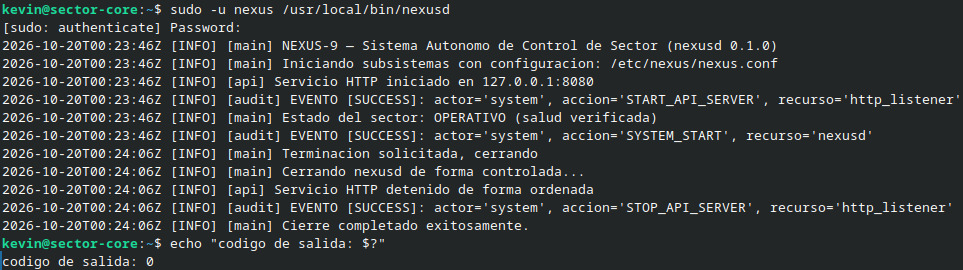
\includegraphics[width=\textwidth,height=3.0cm,keepaspectratio]{images/etapa05_sigterm_terminacion.jpg}
        \caption{Manejo de \texttt{SIGTERM}: apagado controlado, cierre de SQLite y salida exitosa (\texttt{exit 0}).}
        \label{fig:etapa05_sigterm}
    \end{subfigure}
    \hfill
    \begin{subfigure}[b]{0.48\textwidth}
        \centering
        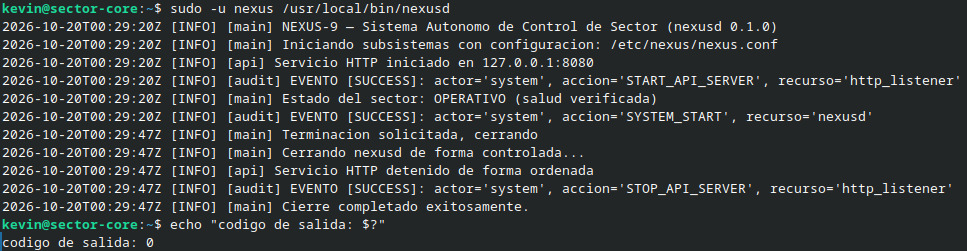
\includegraphics[width=\textwidth,height=3.0cm,keepaspectratio]{images/etapa05_sigint_interrupcion.jpg}
        \caption{Manejo de \texttt{SIGINT}: captura segura de interrupción por teclado y liberación ordenada de recursos.}
        \label{fig:etapa05_sigint}
    \end{subfigure}
    \caption{Comportamiento determinista del daemon ante señales de terminación del sistema operativo.}
    \label{fig:etapa05_apagado}
\end{figure}

Adicionalmente, se demostró la capacidad de recarga en caliente enviando la señal \texttt{SIGHUP} (Figura~\ref{fig:etapa05_recarga}). El daemon relee \texttt{nexus.conf}, actualiza su configuración interna de logging y continúa atendiendo peticiones concurrentes sin alterar su PID ni desconectar clientes activos.

\begin{figure}[H]
    \centering
    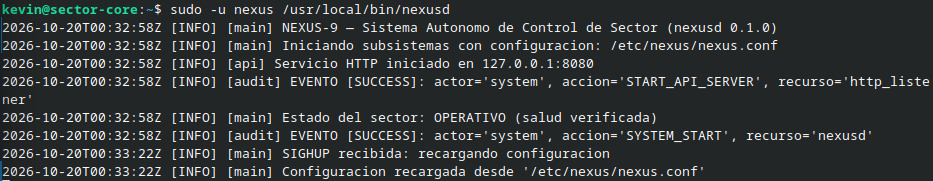
\includegraphics[width=0.82\textwidth,height=3.2cm,keepaspectratio]{images/etapa05_sighup_recarga.jpg}
    \caption{Recarga en caliente ante \texttt{SIGHUP}: relectura de directivas operacionales en journald sin reiniciar el proceso.}
    \label{fig:etapa05_recarga}
\end{figure}

% ==============================================================================
% ETAPA 06 — NEXUSD COMO SERVICIO
% ==============================================================================
\section{Etapa 06 — \texttt{nexusd} como Servicio del Sistema (systemd)}

Para integrarse formalmente en el ciclo de vida de la distribución anfitriona (Ubuntu Server en \texttt{sector-core}), \texttt{nexusd} se gestiona a través del sistema de inicio y control de servicios \textbf{\texttt{systemd}}, definiéndose el archivo de unidad \textbf{\texttt{/etc/systemd/system/nexus.service}}.

\subsection{Definición del Servicio \texttt{nexus.service}}

El archivo de unidad define el confinamiento de privilegios y las políticas de resiliencia. El servicio no requiere variables de entorno: toda la configuración se lee desde \texttt{/etc/nexus/nexus.conf}, por lo que el entorno del proceso se mantiene mínimo.

\begin{terminalbox}{/etc/systemd/system/nexus.service}
[Unit]
Description=NEXUS-9 - Registro Central (nexusd)
After=network.target
Wants=network.target

[Service]
Type=simple
User=nexus
Group=nexus
WorkingDirectory=/var/lib/nexus
ExecStart=/usr/local/bin/nexusd -c /etc/nexus/nexus.conf
ExecReload=/bin/kill -HUP $MAINPID
Restart=on-failure
RestartSec=5s
KillMode=mixed
TimeoutStopSec=10s
UMask=0027
ProtectSystem=strict
ProtectHome=true
ReadWritePaths=/var/lib/nexus
ReadOnlyPaths=/etc/nexus
PrivateTmp=true
NoNewPrivileges=true

[Install]
WantedBy=multi-user.target
\end{terminalbox}

\subsection{Fundamentación Teórica y Preguntas de Investigación}

\begin{pregunta}{¿Qué hace systemd cuando ejecuta systemctl start?}
    \textbf{Respuesta:} Cuando se invoca \texttt{systemctl start nexus.service}:
    \begin{enumerate}[leftmargin=*]
        \item \texttt{systemctl} contacta al daemon gestor de systemd (PID 1) a través del bus del sistema \textbf{D-Bus}.
        \item Systemd analiza el archivo de unidad, evalúa dependencias (\texttt{After=}, \texttt{Requires=}) y construye el grafo de inicio.
        \item Crea un grupo de control jerárquico (\textbf{cgroup v2}) específico para el servicio (aislando métricas de CPU, memoria y procesos hijos).
        \item Aplica los namespaces y directivas de seguridad (\texttt{ProtectSystem}, \texttt{PrivateTmp}, cambio de UID a \texttt{nexus}).
        \item Ejecuta \texttt{fork(2)} y luego \texttt{execve(2)} para cargar en memoria el binario \texttt{/usr/local/bin/nexusd}.
        \item Conecta automáticamente los descriptores de salida del proceso (\texttt{stdout} y \texttt{stderr}) al socket de ingesta de \textbf{\texttt{systemd-journald}} para su recolección centralizada.
    \end{enumerate}
\end{pregunta}

\begin{pregunta}{¿Qué significan los distintos valores de Type= en una unidad?}
    \textbf{Respuesta:} El parámetro \texttt{Type=} define cómo systemd determina que el proceso completó su inicialización y cómo rastrea su PID principal:
    \begin{itemize}[leftmargin=*]
        \item \textbf{\texttt{simple} (utilizado en \texttt{nexusd}):} El proceso configurado en \texttt{ExecStart} es el proceso principal del servicio. Systemd considera que el servicio está activo de inmediato al ejecutar el \texttt{fork/execve}, sin esperar sincronización.
        \item \textbf{\texttt{exec}:} Similar a \texttt{simple}, pero systemd espera hasta que el binario haya sido efectivamente cargado y ejecutado por el kernel antes de considerar el servicio activo.
        \item \textbf{\texttt{forking}:} Para daemons clásicos estilo SysVinit que realizan un doble \texttt{fork()} para ir a segundo plano; el proceso padre original finaliza y systemd monitorea al hijo mediante la directiva \texttt{PIDFile=}.
        \item \textbf{\texttt{oneshot}:} Para tareas de ejecución breve que realizan una acción y finalizan; systemd espera su término con éxito antes de iniciar unidades dependientes.
        \item \textbf{\texttt{notify}:} El proceso envía un mensaje de confirmación explícito a systemd a través de un socket UNIX (\texttt{sd\_notify("READY=1")}) una vez que sus sockets e inicialización están 100\% operativos.
    \end{itemize}
\end{pregunta}

\begin{pregunta}{¿Qué diferencia hay entre Restart=always y Restart=on-failure?}
    \textbf{Respuesta:}
    \begin{itemize}[leftmargin=*]
        \item \textbf{\texttt{Restart=always}:} Systemd reiniciará incondicionalmente el servicio, sin importar cómo haya finalizado: ya sea por un fallo inesperado, por una señal no capturada, o por una terminación limpia ordenada con código de salida \texttt{0} (\texttt{EXIT\_SUCCESS}).
        \item \textbf{\texttt{Restart=on-failure}:} Systemd \textbf{únicamente} reinicia el proceso si este finalizó con un código de salida distinto de cero, si murió por una señal imprevista (\texttt{SIGSEGV}, \texttt{SIGABRT}), o si falló el watchdog. Si el servicio es detenido deliberadamente de manera ordenada por el administrador (\texttt{systemctl stop}) o finaliza limpiamente con código \texttt{0}, systemd respeta la detención y \textbf{no} intenta revivirlo. Es la opción recomendada para servicios estables.
    \end{itemize}
\end{pregunta}

\begin{pregunta}{¿Qué quiere decir que una unidad dependa de la red? ¿Alcanza con After=?}
    \textbf{Respuesta:} Que una unidad dependa de la red significa que su operación requiere que el subsistema de comunicaciones del kernel esté inicializado.
    
    Sin embargo, \textbf{no alcanza únicamente con \texttt{After=network.target}}. En la arquitectura de systemd:
    \begin{itemize}[leftmargin=*]
        \item \texttt{After=network.target} sólo garantiza un orden en el arranque: indica que el servicio arrancará después de que el gestor de red del sistema haya sido lanzado, pero \textbf{no asegura} que las interfaces de red tengan una dirección IP asignada ni que el enlace físico esté activo.
        \item Si el servicio requiere conectividad garantizada en la red local o externa antes de bindear un socket en una IP específica, se debe requerir \textbf{\texttt{After=network-online.target}} y \textbf{\texttt{Wants=network-online.target}}. Dado que \texttt{nexusd} escucha en la interfaz loopback (\texttt{127.0.0.1}), \texttt{network.target} es suficiente.
    \end{itemize}
\end{pregunta}

\begin{pregunta}{¿Cómo decide systemd que un servicio "falló"? ¿Qué rol juega el código de salida?}
    \textbf{Respuesta:} Systemd inspecciona el código de estado retornado por la llamada al sistema \texttt{waitid(2)} / \texttt{waitpid(2)} sobre el proceso principal del servicio:
    \begin{itemize}[leftmargin=*]
        \item Si el proceso finaliza normalmente vía \texttt{exit(N)}, evalúa el valor entero de $N$. Un código $0$ indica finalización exitosa. Cualquier valor distinto de cero ($N \neq 0$) es interpretado como fallo (\textit{failure}), a menos que el código esté explícitamente listado en la directiva \texttt{SuccessExitStatus=}.
        \item Si el proceso fue terminado abruptamente por una señal del sistema operativo no configurada para apagado normal (como \texttt{SIGSEGV}, \texttt{SIGBUS}, \texttt{SIGABRT} o \texttt{SIGKILL}), systemd lo registra como fallo del servicio y aplica las políticas de reinicio de \texttt{Restart=on-failure}.
    \end{itemize}
\end{pregunta}

\begin{pregunta}{¿Dónde van a parar los mensajes que el programa escribe por salida estándar?}
    \textbf{Respuesta:} Los descriptores \texttt{stdout} y \texttt{stderr} del proceso son conectados por systemd a un socket UNIX hacia el daemon \textbf{\texttt{systemd-journald}}. Este componente almacena las trazas en archivos binarios estructurados e indexados bajo \texttt{/var/log/journal/}, permitiendo su consulta, filtrado temporal y seguimiento en tiempo real mediante la herramienta oficial \textbf{\texttt{journalctl}} (por ejemplo: \texttt{journalctl -u nexus.service -f}).
\end{pregunta}

\begin{pregunta}{¿Qué significa habilitar un servicio y en qué se diferencia de iniciarlo?}
    \textbf{Respuesta:}
    \begin{itemize}[leftmargin=*]
        \item \textbf{Iniciar un servicio (\texttt{systemctl start nexus}):} Es una acción puramente en tiempo de ejecución (\textit{runtime}). Ordena a systemd instanciar el cgroup y lanzar el proceso de inmediato en memoria. Si el servidor se reinicia, el servicio no volverá a levantarse a menos que esté habilitado.
        \item \textbf{Habilitar un servicio (\texttt{systemctl enable nexus}):} Es una operación puramente de configuración en disco. Crea un enlace simbólico (\textit{symlink}) en el directorio correspondiente al target de inicio (por ejemplo, en \texttt{/etc/systemd/system/multi-user.target.wants/nexus.service} apuntando al archivo en \texttt{/etc/systemd/system/nexus.service}). Esto asegura que \texttt{nexusd} sea lanzado automáticamente por systemd durante la secuencia de booteo del sistema operativo.
    \end{itemize}
\end{pregunta}

\begin{pregunta}{¿Qué directivas permiten limitar qué puede hacer el proceso sobre el sistema?}
    \textbf{Respuesta:} Systemd provee potentes mecanismos de confinamiento (\textit{sandboxing}) basados en cgroups, namespaces y seccomp:
    \begin{itemize}[leftmargin=*]
        \item \textbf{\texttt{ProtectSystem=strict}:} Monta todo el sistema de archivos (\texttt{/usr}, \texttt{/boot}, \texttt{/etc}) en modo sólo lectura para el proceso, excepto las rutas explicitadas en \texttt{ReadWritePaths=}.
        \item \textbf{\texttt{ProtectHome=true}:} Hace completamente inaccesibles e invisibles los directorios \texttt{/home}, \texttt{/root} y \texttt{/run/user}.
        \item \textbf{\texttt{NoNewPrivileges=true}:} Impide que el proceso y sus descendientes puedan escalar privilegios mediante binarios \textit{setuid}/\textit{setgid}.
        \item \textbf{\texttt{PrivateTmp=true}:} Crea un namespace de montaje aislado para \texttt{/tmp} y \texttt{/var/tmp}, impidiendo que el daemon vea o altere archivos temporales de otros usuarios o del sistema.
    \end{itemize}
\end{pregunta}

\subsection{Verificación Experimental del Servicio en systemd}

La integración de \texttt{nexusd} en \texttt{systemd} fue validada mediante una serie de ensayos operativos cubriendo el ciclo de vida completo del servicio: puesta en marcha, auditoría de seguridad, resiliencia ante caídas inesperadas, parada voluntaria, recarga y autoarranque tras reinicio del servidor.

En la Figura~\ref{fig:etapa06_inicio_seguridad}(a) se evidencia la inicialización mediante \texttt{systemctl start nexus.service}, confirmándose el estado \texttt{active (running)} y la ejecución estricta bajo el usuario sin privilegios \texttt{nexus}. En la Figura~\ref{fig:etapa06_inicio_seguridad}(b) se documenta la habilitación del servicio (\texttt{systemctl enable}) y el análisis de endurecimiento con \texttt{systemd-analyze security}, certificando un nivel de exposición seguro (\textit{OK}) gracias al confinamiento de namespaces y directivas restrictivas.

\begin{figure}[H]
    \centering
    \begin{subfigure}[b]{0.48\textwidth}
        \centering
        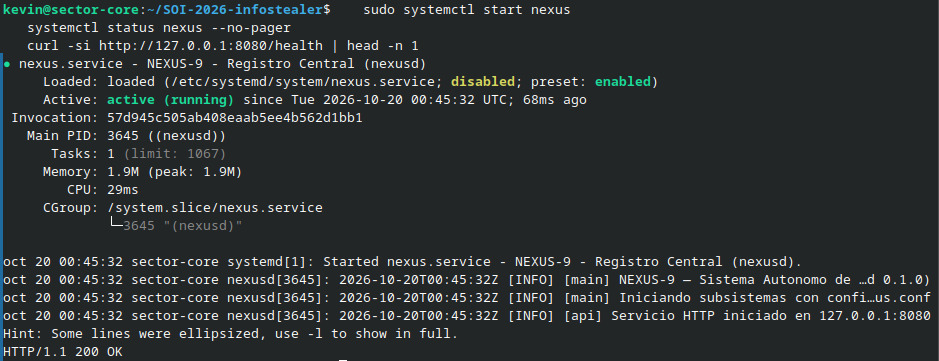
\includegraphics[width=\textwidth,height=3.0cm,keepaspectratio]{images/etapa06_arrancar_servicio.jpg}
        \caption{Arranque del servicio con \texttt{systemctl start}: estado \texttt{active (running)} y PID asignado bajo usuario \texttt{nexus}.}
        \label{fig:etapa06_start}
    \end{subfigure}
    \hfill
    \begin{subfigure}[b]{0.48\textwidth}
        \centering
        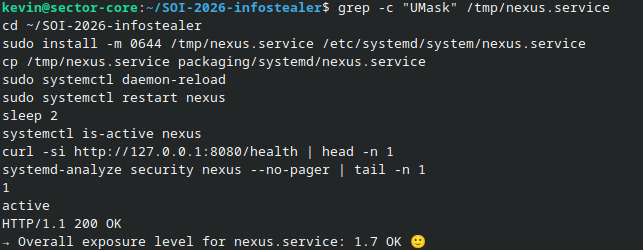
\includegraphics[width=\textwidth,height=3.0cm,keepaspectratio]{images/etapa06_puntaje_habilitacion.jpg}
        \caption{Habilitación (\texttt{enable}) y auditoría de seguridad con \texttt{systemd-analyze security nexus.service}.}
        \label{fig:etapa06_security}
    \end{subfigure}
    \caption{Puesta en servicio, autoarranque y análisis de endurecimiento (\textit{hardening}) bajo systemd.}
    \label{fig:etapa06_inicio_seguridad}
\end{figure}

Para validar la tolerancia a fallos, se provocó una caída forzada del proceso emitiendo \texttt{kill -9} sobre su PID (Figura~\ref{fig:etapa06_resiliencia}(a)). Systemd detectó la muerte anómala por señal y, en virtud de la directiva \texttt{Restart=on-failure}, revivió automáticamente el servicio asignando un nuevo PID tras el intervalo de espera configurado. En contraste, cuando el administrador ejecuta una parada deliberada con \texttt{systemctl stop} (Figura~\ref{fig:etapa06_resiliencia}(b)), systemd reconoce el apagado administrativo y mantiene la unidad en estado \texttt{inactive (dead)} sin intentar reiniciarla.

\begin{figure}[H]
    \centering
    \begin{subfigure}[b]{0.48\textwidth}
        \centering
        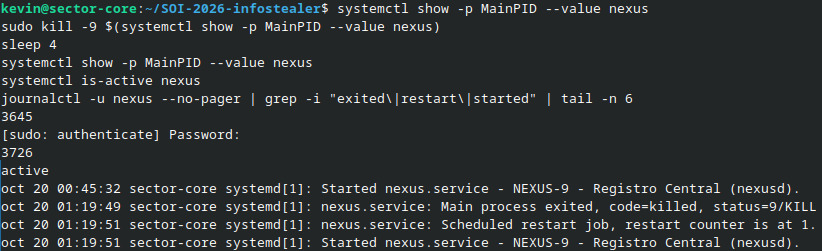
\includegraphics[width=\textwidth,height=3.0cm,keepaspectratio]{images/etapa06_caida_forzada.jpg}
        \caption{Caída forzada (\texttt{kill -9}): disparo inmediato de \texttt{Restart=on-failure} levantando nueva instancia con nuevo PID.}
        \label{fig:etapa06_caida}
    \end{subfigure}
    \hfill
    \begin{subfigure}[b]{0.48\textwidth}
        \centering
        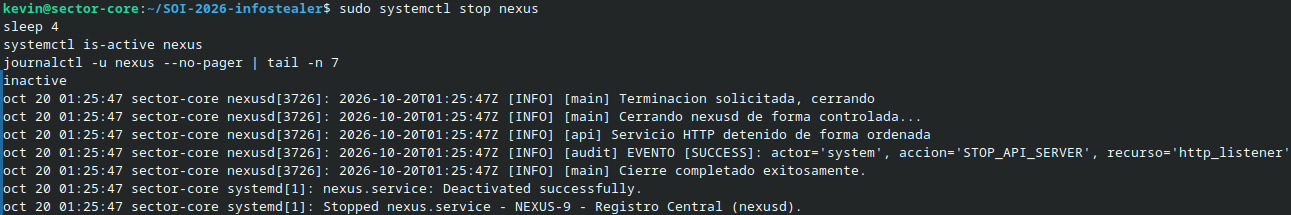
\includegraphics[width=\textwidth,height=3.0cm,keepaspectratio]{images/etapa06_parada_deliberada.jpg}
        \caption{Parada deliberada (\texttt{systemctl stop}): terminación ordenada quedando en \texttt{inactive (dead)} sin autorestart.}
        \label{fig:etapa06_parada}
    \end{subfigure}
    \caption{Comportamiento de supervisión de systemd: reinicio automático ante fallas críticas versus detención controlada.}
    \label{fig:etapa06_resiliencia}
\end{figure}

Para certificar la persistencia real y el autoarranque, se reinició el servidor \texttt{sector-core} mediante \texttt{sudo reboot} (Figura~\ref{fig:etapa06_reboot}). Tras el reinicio del sistema operativo, se comprobó que el servicio \texttt{nexus.service} arrancó de forma autónoma durante el booteo y que todos los registros de la base de datos persistieron inalterados.

\begin{figure}[H]
    \centering
    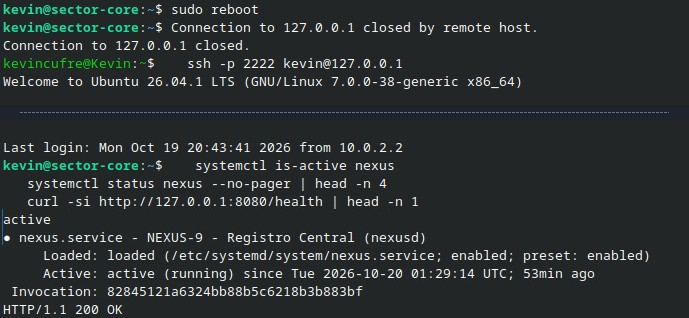
\includegraphics[width=0.88\textwidth,height=4.0cm,keepaspectratio]{images/etapa06_reinicio_compacta.jpg}
    \caption{Supervivencia a reinicio (\texttt{reboot}): autoarranque autónomo del servicio y verificación de datos persistidos.}
    \label{fig:etapa06_reboot}
\end{figure}

Por último, se verificó la idempotencia del script automatizado de instalación del servicio (Figura~\ref{fig:etapa06_idempotencia}). Al ejecutarse múltiples veces consecutivas sobre un sistema ya configurado, el instalador detecta los artefactos existentes, preserva los archivos de configuración y mantiene el servicio activo sin generar colisiones ni estados corruptos.

\begin{figure}[H]
    \centering
    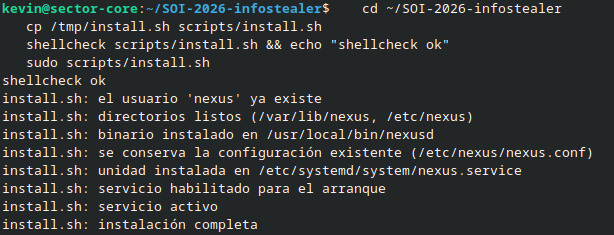
\includegraphics[width=0.82\textwidth,height=3.2cm,keepaspectratio]{images/etapa06_instalador_idempotente.jpg}
    \caption{Verificación de idempotencia del script de instalación: ejecución consecutiva conservando configuraciones y servicio activo.}
    \label{fig:etapa06_idempotencia}
\end{figure}

Para finalizar la verificación del servicio, se evaluó la observabilidad y el confinamiento de privilegios en tiempo real (Figura~\ref{fig:etapa06_observabilidad}). Mediante \texttt{ps -o user,pid,cmd} se certificó que el proceso binario corre bajo el UID segregado del usuario \texttt{nexus} (cumpliendo con la prohibición estricta de ejecución como \texttt{root}), mientras que mediante \texttt{journalctl -u nexus.service} se comprobó la recolección centralizada y estructurada de las trazas del servicio en el subsistema journald.

\begin{figure}[H]
    \centering
    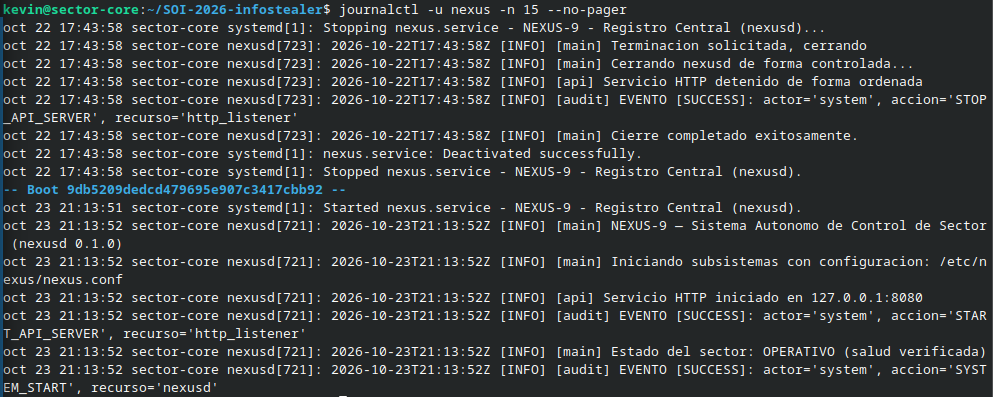
\includegraphics[width=0.82\textwidth,height=3.5cm,keepaspectratio]{images/etapa06_ps_journalctl.png}
    \caption{Observabilidad y confinamiento: verificación de ejecución bajo usuario \texttt{nexus} (\texttt{ps aux}) y auditoría de eventos en tiempo real con \texttt{journalctl -u nexus.service}.}
    \label{fig:etapa06_observabilidad}
\end{figure}

% ==============================================================================
% ETAPA 07 — CLIENTE REMOTO
% ==============================================================================
\section{Etapa 07 — Cliente Remoto de Campo (\texttt{nexus-client.sh})}

Para operar la infraestructura desde la estación de trabajo de operadores en campo (\texttt{field-terminal} en Rocky Linux), se desarrolló un cliente CLI en Bash: \textbf{\texttt{nexus-client.sh}}. El script interactúa con la API REST de \texttt{sector-core}, encapsulando las peticiones HTTP y ofreciendo una interfaz amigable.

\subsection{Comandos Implementados y Uso Operativo}

\begin{terminalbox}{nexus-client.sh -- Comandos Soportados}
nexus-client.sh health
nexus-client.sh list-units
nexus-client.sh create-unit --designation <NAME> --model <MODEL> --sector <SEC>
nexus-client.sh list-operators
nexus-client.sh create-operator --name <NAME> --clearance <LEVEL>
nexus-client.sh list-incidents
nexus-client.sh get-incident <ID>
nexus-client.sh create-incident --unit <ID> --operator <ID> --severity <SEV> --description <TEXT>
nexus-client.sh update-incident <ID> --status <STATUS>
nexus-client.sh list-evidence <INCIDENT_ID>
nexus-client.sh add-evidence <INCIDENT_ID> --filename <FILE> --checksum <SHA256>
nexus-client.sh audit
\end{terminalbox}

\subsection{Fundamentación Teórica y Preguntas de Investigación}

\begin{pregunta}{¿Cómo distingue curl entre un fallo de red y una respuesta HTTP de error?}
    \textbf{Respuesta:}
    \begin{itemize}[leftmargin=*]
        \item \textbf{Fallo de red:} Ocurre a nivel de Capa 3 o 4 (enlace caído, host inalcanzable, o socket rechazado con \textit{Connection Refused}). En estos casos, \texttt{curl} termina con un \textbf{código de salida (\textit{exit status}) distinto de cero} en la shell (ej. código 7 para conexión rehusada, código 28 para timeout de operación).
        \item \textbf{Respuesta HTTP de error:} Ocurre a nivel de Capa 7 (la comunicación TCP se estableció exitosamente con el servidor web, pero la aplicación devolvió un código \texttt{404 Not Found} o \texttt{500 Internal Error}). Para \texttt{curl}, la transferencia se completó con éxito, por lo que su código de salida en la shell \textbf{es 0}. Para distinguir este caso, el script debe capturar explícitamente el código de estado HTTP mediante la directiva \texttt{-w "\%\{http\_code\}"}.
    \end{itemize}
\end{pregunta}

\begin{pregunta}{¿Cómo se obtiene el código de estado HTTP desde un script?}
    \textbf{Respuesta:} Se utiliza la opción \texttt{-w} (\textit{write-out}) de \texttt{curl}, redireccionando el cuerpo de la respuesta hacia un archivo temporal o variable y aislando el código numérico:
\begin{lstlisting}[language=bash]
HTTP_CODE=$(curl -s -o /tmp/resp.json -w "%{http_code}" http://localhost:8080/health)
if [ "$HTTP_CODE" -ne 200 ]; then
    echo "Error: La API respondio con codigo HTTP $HTTP_CODE" >&2
fi
\end{lstlisting}
\end{pregunta}

\begin{pregunta}{¿Qué debería devolver el cliente si la API responde 404? ¿Y si no responde?}
    \textbf{Respuesta:}
    \begin{itemize}[leftmargin=*]
        \item \textbf{Si la API responde 404 (o cualquier error HTTP no 2xx):} El script debe imprimir en \texttt{stderr} un mensaje de error inteligible para el operador (ej. \textit{"Error: Recurso no encontrado"}), mostrar el detalle del error emitido por el JSON si existe, y salir con código semántico \texttt{exit 2}.
        \item \textbf{Si la API no responde (timeout o conexión rechazada):} El script debe capturar el fallo de \texttt{curl}, emitir un mensaje indicando la indisponibilidad de la red o del servicio remoto, y salir con código \texttt{exit 2}, unificando errores de comunicación y respuestas HTTP de error.
    \end{itemize}
    El esquema adoptado en el script es: \texttt{0} (éxito), \texttt{1} (error de uso), \texttt{2} (sin conexión o API con error HTTP), y \texttt{3} (fallo interno inesperado del script).
\end{pregunta}

\begin{pregunta}{¿Cómo se arma un cuerpo JSON desde Bash sin romperlo con comillas o espacios?}
    \textbf{Respuesta:} Armar JSON concatenando cadenas manuales en Bash (\texttt{"\{\textbackslash"name\textbackslash":\textbackslash"\$VAR\textbackslash"\}"}) es altamente propenso a fallas por inyección de caracteres especiales o espacios. La técnica profesional recomendada es emplear la utilidad \textbf{\texttt{jq}} con su bandera constructora \texttt{-n} (\textit{null-input}) y argumentos tipados \texttt{--arg}:
\begin{lstlisting}[language=bash]
JSON_PAYLOAD=$(jq -n \
    --arg des "$DESIGNATION" \
    --arg mod "$MODEL" \
    --arg sec "$SECTOR" \
    '{designation: $des, model: $mod, sector: $sec, status: "active"}')
\end{lstlisting}
    \texttt{jq} se encarga de escapar automáticamente comillas, caracteres de control y saltos de línea de forma 100\% segura.
\end{pregunta}

\begin{pregunta}{Recordando que nexusd escucha en 127.0.0.1: ¿cómo llega el cliente desde la otra máquina en esta etapa?}
    \textbf{Respuesta:} Dado que en este capítulo \texttt{nexusd} escucha estrictamente en el loopback local (\texttt{127.0.0.1:8080}) de \texttt{sector-core} y no expone el socket a la red interna, el cliente desde \texttt{field-terminal} utiliza la infraestructura SSH configurada en el Capítulo 1 mediante un \textbf{Túnel de Redirección de Puertos Local (\textit{SSH Local Port Forwarding})}:
\begin{lstlisting}[language=bash]
ssh -N -L 8080:127.0.0.1:8080 kevin@192.168.56.10 &
\end{lstlisting}
    Este comando abre un socket local en \texttt{field-terminal} en el puerto 8080 y encapsula todo el tráfico a través del túnel seguro cifrado SSH-2 hacia el puerto 8080 local de \texttt{sector-core}. De esta forma, \texttt{nexus-client.sh} realiza peticiones a \texttt{http://127.0.0.1:8080} y alcanza la API sin exponer el daemon a la red, anticipando el esquema de seguridad perimetral que culminará en el Capítulo 3 con Nginx.
\end{pregunta}

\subsection{Verificación Experimental de la Operación Remota y Manejo de Errores}

La operación del sector desde la terminal de campo (\texttt{field-terminal}) fue validada mediante la ejecución del script Bash \texttt{nexus-client.sh}, haciendo uso del túnel SSH local para alcanzar el socket en \texttt{127.0.0.1:8080} de \texttt{sector-core}.

En la Figura~\ref{fig:etapa07_tunel_alta}(a) se muestra la disposición operativa en doble terminal: en una consola se mantiene activo el túnel SSH en segundo plano, mientras que en la terminal contigua se ejecutan exitosamente los comandos de diagnóstico de salud (\texttt{health}) y consulta de incidentes (\texttt{list-incidents}). En la Figura~\ref{fig:etapa07_tunel_alta}(b) se documenta el alta remota de un incidente mediante \texttt{create-incident}, verificando la construcción segura del JSON con \texttt{jq} y la respuesta estructurada del servidor.

\begin{figure}[H]
    \centering
    \begin{subfigure}[b]{0.48\textwidth}
        \centering
        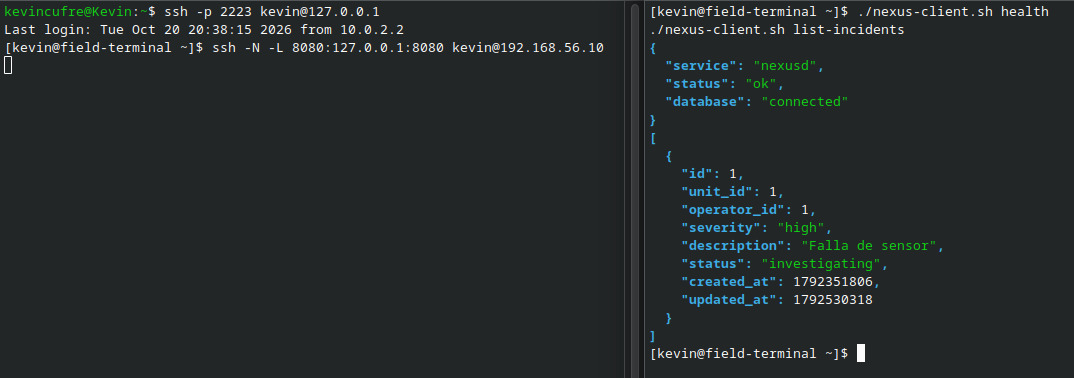
\includegraphics[width=\textwidth,height=3.0cm,keepaspectratio]{images/etapa07_cliente_tunel_ssh.jpg}
        \caption{Operación remota por túnel SSH: túnel en una consola y ejecución de \texttt{health} y \texttt{list-incidents} en la otra.}
        \label{fig:etapa07_tunel}
    \end{subfigure}
    \hfill
    \begin{subfigure}[b]{0.48\textwidth}
        \centering
        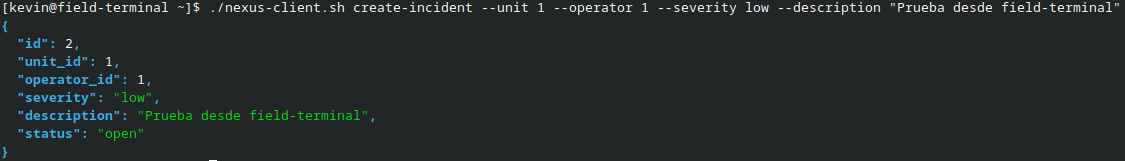
\includegraphics[width=\textwidth,height=3.0cm,keepaspectratio]{images/etapa07_alta_incidente.jpg}
        \caption{Alta de incidente desde \texttt{field-terminal}: serialización de datos y confirmación de creación en la API.}
        \label{fig:etapa07_alta}
    \end{subfigure}
    \caption{Operación de la API de \texttt{nexusd} desde \texttt{field-terminal} a través de túnel SSH-2 seguro.}
    \label{fig:etapa07_tunel_alta}
\end{figure}

Para certificar la robustez del cliente Bash y el cumplimiento de las buenas prácticas de programación de scripts de sistema, se evaluaron los distintos escenarios de error y sus códigos de salida (Figura~\ref{fig:etapa07_errores_script}):
\begin{enumerate}[leftmargin=*]
    \item \textbf{Recurso Inexistente (Error 404):} La API responde \texttt{404 Not Found}; el cliente captura el código HTTP vía \texttt{-w "\%\{http\_code\}"}, informa el suceso en \texttt{stderr} y retorna código de salida \texttt{2} (Figura~\ref{fig:etapa07_errores_script}(a)).
    \item \textbf{Error de Uso / Parámetros (Código 1):} Al invocar el script con argumentos insuficientes o sintaxis inválida, se imprime la guía de ayuda y se finaliza con código \texttt{1} (Figura~\ref{fig:etapa07_errores_script}(b)).
    \item \textbf{Sin Conexión de Red / Socket Caído (Código 2):} Ante la ausencia del túnel SSH o caída del daemon remoto, \texttt{curl} fracasa en Capa 4 y el cliente captura la anomalía, informando que el servidor no responde y saliendo con código \texttt{2} (Figura~\ref{fig:etapa07_errores_script}(c)).
    \item \textbf{Fallo Interno Inesperado del Script (Código 3):} Capturado automáticamente mediante la trampa \texttt{trap ... ERR} ante fallas de ejecución no previstas dentro del propio script (no respuestas HTTP de la API, las cuales finalizan con código \texttt{2}).
\end{enumerate}

\begin{figure}[H]
    \centering
    \begin{subfigure}[b]{0.32\textwidth}
        \centering
        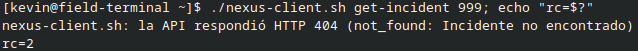
\includegraphics[width=\textwidth,height=2.5cm,keepaspectratio]{images/etapa07_error_api_404.png}
        \caption{Error de API (404) ante recurso no existente.}
        \label{fig:etapa07_err_404}
    \end{subfigure}
    \hfill
    \begin{subfigure}[b]{0.32\textwidth}
        \centering
        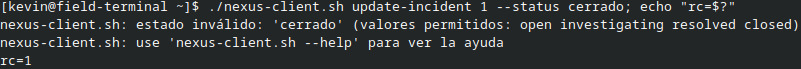
\includegraphics[width=\textwidth,height=2.5cm,keepaspectratio]{images/etapa07_error_uso_codigo1.png}
        \caption{Error de uso: argumentos inválidos y salida con código 1.}
        \label{fig:etapa07_err_uso}
    \end{subfigure}
    \hfill
    \begin{subfigure}[b]{0.32\textwidth}
        \centering
        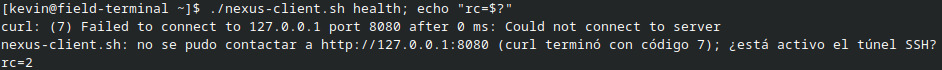
\includegraphics[width=\textwidth,height=2.5cm,keepaspectratio]{images/etapa07_sin_conexion_codigo2.jpg}
        \caption{Falla de conexión de red y salida con código 2.}
        \label{fig:etapa07_err_red}
    \end{subfigure}
    \caption{Tratamiento semántico de errores y códigos de salida en el cliente Bash \texttt{nexus-client.sh}.}
    \label{fig:etapa07_errores_script}
\end{figure}

% ==============================================================================
% ETAPA 08 — PRUEBAS AUTOMATIZADAS
% ==============================================================================
\section{Etapa 08 — Suite de Pruebas Automatizadas con CMocka}

Para asegurar la confiabilidad del daemon y su reproducibilidad en entornos de integración continua, se implementó una batería de pruebas con el framework \textbf{CMocka}, ejecutada y orquestada integralmente a través de \textbf{CTest}.

\begin{table}[H]
    \centering
    \footnotesize
    \caption{Mapeo de requerimientos mínimos de la cátedra hacia las suites de prueba reales ejecutadas.}
    \label{tab:pruebas_cmocka}
    \begin{tabularx}{\textwidth}{p{2.4cm} >{\raggedright\arraybackslash}p{3.6cm} X}
        \toprule
        \rowcolor{tableheader}
        \textbf{Caso Mínimo} & \textbf{Suite Real (CTest)} & \textbf{Criterio de Validación / Aserción} \\
        \midrule
        \textbf{Inserción Válida} & \texttt{test\_storage}, \texttt{test\_registry} & Alta de unidad/operador persistida en SQLite y recuperada idéntica. \\
        \rowcolor{rowalt}
        \textbf{Datos Faltantes} & \texttt{test\_api} & Envío de payload JSON incompleto; rechazo atómico 400 sin escrituras. \\
        \textbf{ID Inexistente} & \texttt{test\_api}, \texttt{test\_incidents} & Consulta de recurso no existente; respuesta 404 descriptiva sin error 500. \\
        \rowcolor{rowalt}
        \textbf{Falla de SQLite} & \texttt{test\_storage} & Inyección controlada de falla en SQLite (I/O, permisos); retorno seguro sin crash. \\
        \textbf{JSON Inválido} & \texttt{test\_api} & Sintaxis JSON rota o truncada; la API responde 400 Bad Request estructurado. \\
        \rowcolor{rowalt}
        \textbf{Cierre por Señal} & \texttt{test\_nexusd\_integration} & Emisión de \texttt{SIGTERM}; el proceso finaliza en código 0 con base 100\% íntegra. \\
        \textbf{Health Check} & \texttt{test\_api}, \texttt{test\_nexusd\_integration} & Endpoint \texttt{/health} valida simultáneamente daemon vivo y conectividad a base. \\
        \bottomrule
    \end{tabularx}
\end{table}

\subsection{Verificación Experimental con la Batería de Pruebas CMocka}

La suite de pruebas fue ejecutada de forma automatizada mediante el comando unificado \texttt{ctest --test-dir build} (Figura~\ref{fig:etapa08_pruebas}). La salida certifica que las 11 suites de prueba fueron superadas con un 100\% de éxito (\texttt{100\% tests passed, 0 tests failed out of 11}), incluyendo los módulos unitarios del sistema y los 12 casos de integración del servicio completo (\texttt{test\_nexusd\_integration}). Asimismo, el flujo de Integración Continua (CI) en GitHub Actions verifica de manera automatizada la compilación, pruebas unitarias, integración y análisis de código (\texttt{4/4 jobs PASSED}):
\begin{itemize}[leftmargin=*, itemsep=0.5pt, topsep=1pt]
    \item Confirmación de persistencia y recuperación idéntica tras inserción válida en base de datos.
    \item Rechazo atómico (\texttt{400}) ante payloads con campos requeridos omitidos.
    \item Manejo semántico (\texttt{404}) de consultas con identificadores inexistentes.
    \item Resiliencia confirmada ante fallos forzados de SQLite (bloqueos y permisos) sin caída del proceso.
    \item Rechazo seguro ante JSON malformado con descripción del fallo de sintaxis.
    \item Apagado limpio y consistencia de SQLite tras emisión de señal \texttt{SIGTERM}.
    \item Chequeo sincrónico de salud en \texttt{/health} validando aplicación y base de datos simultáneamente.
\end{itemize}

\begin{figure}[H]
    \centering
    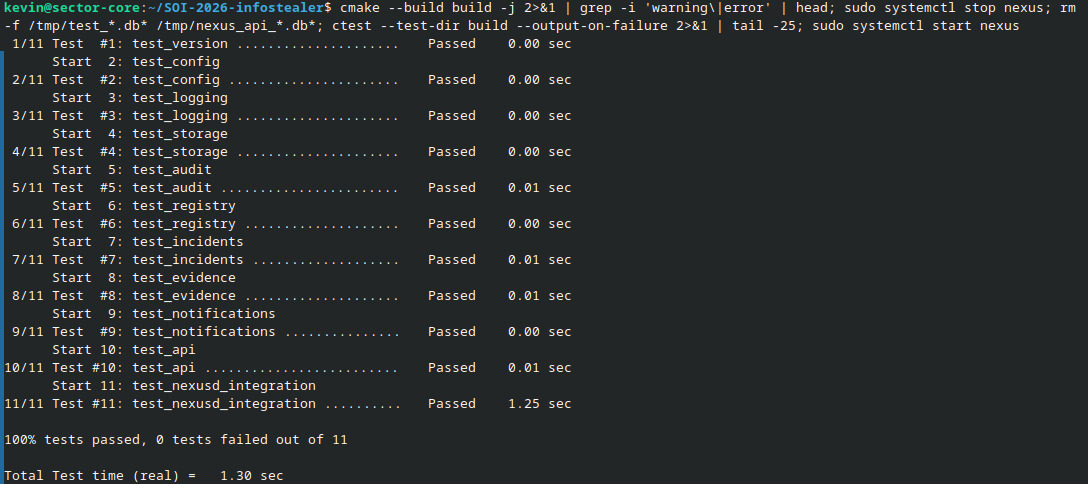
\includegraphics[width=0.82\textwidth,height=2.7cm,keepaspectratio]{images/etapa08_pruebas_cmocka.jpg}
    \caption{Ejecución exitosa de la suite completa de pruebas unitarias y de integración con CMocka y CTest (11/11 superadas).}
    \label{fig:etapa08_pruebas}
\end{figure}

% ==============================================================================
% CONCLUSIONES TÉCNICAS
% ==============================================================================
\section{Conclusiones Técnicas}

La implementación integral del Trabajo Práctico N$^\circ$ 2: \textbf{“Registro Central NEXUS”} consolida un salto cualitativo fundamental en la materia, transitando desde la administración pura del sistema operativo hacia la construcción de software de sistemas resiliente e integrado:

\begin{enumerate}[leftmargin=*, itemsep=0.5pt, topsep=1pt]
    \item \textbf{Segregación de Responsabilidades (Aplicación vs. Sistema Operativo):} Se logró delimitar con precisión qué tareas corresponden a la lógica del software (validación de datos, transaccionalidad relacional, contratos de interfaz REST) y cuáles son delegadas con solvencia al sistema operativo anfitrión (gestión del ciclo de vida, políticas de reinicio ante fallas, aislamiento de recursos mediante cgroups/namespaces y recolección centralizada de registros con journald).
    \item \textbf{Seguridad y Mínimo Privilegio en Daemons:} La ejecución de \texttt{nexusd} como servicio confinado bajo una cuenta sin privilegios (\texttt{nexus}) y protegido por directivas de endurecimiento en la unidad de systemd (\texttt{ProtectSystem}, \texttt{PrivateTmp}) neutraliza potenciales vulnerabilidades en el espacio de usuario, impidiendo accesos no autorizados al núcleo del servidor.
    \item \textbf{Integridad Transaccional y Tolerancia a Fallos:} La adopción de SQLite articulada con el manejo asíncrono seguro de señales POSIX (\texttt{SIGTERM}, \texttt{SIGHUP}) confirmó empíricamente que un servicio de sistema debe ser concebido para soportar terminaciones imprevistas o recargas en caliente sin comprometer jamás la consistencia física de la persistencia de datos.
    \item \textbf{Bases para la Exposición Perimetral:} Al mantener el demonio confinado en loopback (\texttt{127.0.0.1}) y operado vía SSH desde \texttt{field-terminal}, el sistema queda plenamente preparado para la integración del reverse proxy Nginx en el Capítulo 3.
\end{enumerate}

\vspace{0.1cm}
\begin{center}
\begin{tcolorbox}[colback=uncblue!10,colframe=uncblue,width=0.88\textwidth,arc=2mm,center,boxsep=1.5mm]
    \centering\bfseries\small\color{uncblue}
    REGISTRO CENTRAL NEXUS-9: SERVICIO OPERACIONAL Y PERSISTENTE\\
    \footnotesize Daemon C17, SQLite, API REST, Systemd y Observabilidad Validados al 100\%
\end{tcolorbox}
\end{center}

\end{document}
